\chapter{Arbeitspunkt-Regelung}\label{cha:apr}

Nachdem im letzten Kapitel die Modellierung des Gesamtsystems erläutert wurde, stellt sich nun die Frage, wie sich das System regeln lässt. Dabei geht es einerseits um die Regelung an den 4 Arbeitspunkten \siehe{\secref{sec:aps}}, \dah das Stabilisieren und Halten dieser, sowie um \traj n, die das \dpd\ von einem \ap\ in einen anderen überführen (siehe folgendes \charef{cha:trj}).

Alle \ap -Regelungen vergangener Arbeiten basieren auf einer \lin\ und der anschließenden Auslegung eines \ricc-Reglers.
Die Güteparameter wurden dabei jedes Mal anders und meist heuristisch bestimmt.
Da am Versuchsstand nicht alle Zustände gemessen werden können, wurden meistens \beob\ mit Polplatzierung ausgelegt.
Kämmerer \cite{kämmerer} verglich diesen mit einem Zustandsvariablenfilter, mit welchem allerdings keine zufriedenstellende Ergebnisse gelangen.
Apprich \cite{apprich} und Kämmerer \cite{kämmerer} setzten Störgrößenbeobachter ein, die in den folgenden Arbeiten nicht mehr verwendet wurden.
Alle Arbeiten setzten Vorsteuerungsmethoden ein, da die \crb\ am Schlitten bei der Regelung stets problematisch war.
Chang \cite{chang} erstellte ein Simulationsmodell zur \ap-Regelung, das als Orientierung dient.

Beim Reglerentwurf wird zunächst dem Vorgehen vergangener Arbeiten gefolgt. 
Einzelne Aspekte in der Steuerung/Regelung werden anschließend verbessert.
Die Reglerparameter der vorigen Arbeiten werden überprüft und optimiert.
Außerdem wird der Einfluss des \beob\ analysiert.

\begin{figure}[h]
	\centering
		\includegraphics[width=0.42\textwidth]{Bilder/Regelung Vorgehen weiß.pdf}
	\caption{Vorgehen bei der AP-Regelung }
	\label{fig:regvorg}
\end{figure}

\figref{fig:regvorg} stellt das prinzipielle Vorgehen bei der Untersuchung und Optimierung der \ap-Regelung dar.
Es werden zunächst Auswertungsmethoden implementiert, die einzelne Simulationstests evaluieren.
Mit den Anfangswerttests wird das Ermitteln der maximalen Winkelabweichung, ab welcher das System nicht mehr stabilisiert werden kann, automatisiert.
Dadurch können im nächsten Schritt die Reglerparameter systematisch optimiert werden.
Kann dadurch keine gute Regelung erzielt werden, müssen beim Reglerentwurf möglicherweise andere Verfahren eingesetzt werden.
Abschließend wird die Regelbarkeit in Abhängigkeit der Systemparameter untersucht.

Regler können nach verschiedenen Gesichtspunkten wie Dynamik, Überschwingen, Energieverbrauch optimiert werden.
In dieser Arbeit wird bei der Untersuchung und Optimierung des \dpd s stets die Stabilität priorisiert.
Die Optimierung des Einschwingvorgangs steht nicht im Vordergrund.
Daher werden vor allem die instabilen \ap e 2, 3 und 4 untersucht.
Außerdem werden hauptsächlich die maximalen \emph{Winkel}abweichungen betrachtet, da diese wesentlich für die Stabiltät sind.
Die Regelung von Positionsabweichungen wird nachrangig behandelt.


\section{System-\lin\ und Analyse}%\label{sec:}

Das nicht-lineare System wird zunächst linearisiert, dessen \ewe\ analysiert, sowie auf Steuer- und Beobachtbarkeit überprüft.

\subsection{\lin}\label{subsec:lin}

Da das \zrm\ des \spds s \eqref{eq:zrm} nicht-linear ist, muss es um jeden \ap\ linearisiert werden, bevor lineare Regelungsmethoden angewandt werden können. 

\begin{align}
	\mat{A} &= \left. \frac{\partial \vef(\vex,u_R)}{\partial \vex} \right|_{\vex=\vexr}  
		= \left. \begin{bmatrix}
		0 & 1 & 0 & 0 & 0 & 0 \\
		0 & \partiald{a_2(\vex)}{\xop} & \partiald{a_2(\vex)}{\phe} & \partiald{a_2(\vex)}{\phep} & \partiald{a_2(\vex)}{\phz} & \partiald{a_2(\vex)}{\phzp} \\
		0 & 0 & 0 & 1 & 0 & 0 \\
		0 & \partiald{a_4(\vex)}{\xop} & \partiald{a_4(\vex)}{\phe} & \partiald{a_4(\vex)}{\phep} & \partiald{a_4(\vex)}{\phz} & \partiald{a_4(\vex)}{\phzp} \\
		0 & 0 & 0 & 0 & 0 & 1 \\
		0 & \partiald{a_6(\vex)}{\xop} & \partiald{a_6(\vex)}{\phe} & \partiald{a_6(\vex)}{\phep} & \partiald{a_6(\vex)}{\phz} & \partiald{a_6(\vex)}{\phzp} \\
	\end{bmatrix} \right._{\vex=\vexr}  \\
	\mat{B} &= \left. \frac{\partial \vef(\vex_R,u)}{\partial u} \right|_{u=u_R}
	= \ve{b}(\vexr) = \begin{bmatrix}
		0 \\ b_2(\vexr) \\ 0 \\  b_4(\vexr) \\ 0 \\  b_6(\vexr)
	\end{bmatrix}
\end{align}

Somit ergeben sich für jeden \ap\ unterschiedliche Systemmatrizen \mat{A} und Eingangsmatrizen \ve{B}. Beim \bss\ fällt zusätzlich die zweite Zeile und die zweite Spalte (bis auf die 1) weg, da dort $a_2=0$ ist und keine Abhängigkeit von \xop\ besteht \siehe{\tabref{tab:abh}}, außerdem ist $b_2=1$.
Die Ausgangsmatrix \mat{C} ist immer gleich, da die Ausgangsgleichung \eqref{eq:hx} linear ist.

Für den tatsächlichen Zustand wird der \ap-Zustand des linearisierten Systems \dvex\ zum \ap\ addiert:
\begin{subequations} \label{eq:aptransf} \begin{align} 
	\vex(t)&= \vexr + \dvex(t)	\\
	u(t)&= u_R + \Delta u(t)	
\end{align} \end{subequations} 


\subsection{Eigenwerte}\label{sec:ew}

Anhand der \ewe\ können Aussagen über die Dynamik eines Systems getroffen werden. 
Das \bss\ hat aufgrund der zweifachen Integration des Eingangs \xopp\ stets zwei \ewe\ in 0. 
Mit den Apprich-Parametern ergeben sich folgende \ewe:

\begin{table}[htbp]
	\centering
	\caption{\ewe\ des \bss s (Parameter: Apprich)}
		\begin{tabular}[t]{cccc}
			\toprule
			\ape & \apz & \apd & \apv \\
			\midrule
			$0$	&	$0$	&	$0$	&	$0$	\\
			$0$	&	$0$	&	$0$	&	$0$	\\
			$-0.2972 +11.4177\iu$ &    $7.8028						$	&	  $6.8596							$	&   $11.1308$	\\
			$-0.2972 -11.4177\iu$ &   $-7.9367						$	&   $-7.2314					$		&  $-11.7251$	\\
			$-0.0418 + 4.8515\iu$ &   $-0.1858 + 7.0392\iu$	&  $-0.0669 + 7.8676\iu$	&  $  4.8089$	\\
			$-0.0418 - 4.8515\iu$ &   $-0.1858 - 7.0392\iu$	& $ -0.0669 - 7.8676\iu	$	&  $ -4.8926$	\\
			\bottomrule
		\end{tabular}
	\label{tab:ewappr}
\end{table}
Im \ap\ 1 ergeben sich zwei konjugiert-komplexe Polpaare, die sich physikalisch mit der Schwingung der beiden Pendel begründen lassen. Sie befinden sich aufgrund der Dämpfung in der linken s-Halbebene, es ist der einzige stabile \ap. \ap\ 2 und 3 besitzen jeweils ein konjugiert-komplexes Polpaar, da dort das erste \bzw zweite Pendel nach unten zeigt und damit \qq{stabil} ist. Der Realteil ist bei \ap\ 3 deutlich kleiner, was auf die geringere Dämpfung des zweiten Pendelgelenks zurückzuführen ist (siehe \tabref{tab:spdparams}). Aufgrund der Instabilität des anderen Pendels ergibt sich jeweils ein positiv reeller \ew. In \ap\ 4 stehen beide Pendel oben, weswegen es dort zwei \ewe\ in der rechten s-Halbebene gibt.

\begin{table}[htbp]
	\centering
	\caption{\ewe\ des \bss s (Parameter: Ribeiro)}
		\begin{tabular}[t]{cccc}
			\toprule
			\ape & \apz & \apd & \apv \\
			\midrule
				$0$	&	$0$	&	$0$	&	$0$	\\
				$0$	&	$0$	&	$0$	&	$0$	\\
				$-174.3727$						&	$-172.9211$	&	$-173.2473$						&	$-175.4362$	\\
				$-0.3493$							&	$-0.3494$		&	$0.3471$							&	$0.3471$	\\
				$-0.6385 + 7.1578\iu$	&	$6.7715$		&	$-0.6443 + 7.2040\iu$	&	$6.7469$	\\
				$-0.6385 - 7.1578\iu$	&	$-7.6900$ 	&	$-0.6443 - 7.2040\iu$ &	$-7.6570$ \\
			\bottomrule
		\end{tabular}
	\label{tab:ewribe}
\end{table}

Mit den neuen Parametern (Ribeiro) ergibt sich ein anderes Bild (siehe \tabref{tab:ewribe}).
Bei \ap\ 1 und 2 verschwindet ein Polpaar, welches dem ersten Pendel zugeordnet wurde. Ein sehr schneller \ew\ kommt hinzu, außerdem ein langsamer reeller, der bei \ap\ 3 und 4 positiv ist. 
Die Ursache für diese Änderung liegt vermutlich in der Modellierung der \crb\ (siehe \secref{sec:crb}). Bei der \lin\ um die Ruhelage wird die Annäherungsfunktion der \mrm{signum}-Funktion um 0 linearisiert, wo sie sehr steil ist. Dies resultiert in einer sehr hohen Dämpfung. Daher ist es sinnvoll, die \crb\ der Pendelstäbe für den AP-Reglerentwurf zu vernachlässigen.
Wird die \crb\ zu 0 gesetzt, ergeben sich prinzipiell ähnliche Werte wie in \tabref{tab:ewappr}.


\subsection{Steuerbarkeit und Beobachtbarkeit}

Voraussetzung für eine Regelung ist die Steuerbarkeit des Systems. Diese kann für lineare Systeme oder linearisierte Systeme an einem \ap\ mit dem Steuerbarkeitskriterium nach \textsc{Kalman} überprüft werden \cite{AdamyRT2}. Außerdem sollte ein System beobachtbar sein, falls nicht alle Zustände bekannt sind und daher über einen Beobachter ermittelt werden.

Das \spds\ (\bss) ist an allen 4 \ap en vollständig steuer- und beobachtbar.


\section{Aufbau der Regelung}\label{sec:aufbaureg}

Die Aufgabe eines Reglers \bzw einer (Vor-)Steuerung ist es nun, anhand der Messgrößen $\vey=(\xo\ \phe\ \phz)^{\transp}$ \eqref{eq:hx} eine geeignete Steuerspannung $U_{\mrm{Steuer}}$ an den Motor vorzugeben. Dabei teilt sich die Steuerung/Regelung in mehrere Schritte auf. 

Die eigentliche Regelung bildet ein \zsr, welcher entweder am \krs\ oder am \bss\ ausgelegt ist. 
Dessen Stellgröße kann im ersten Fall (\fsoll) direkt an die Motorvorsteuerung gegeben werden.
Beim Beschleunigungssystem muss die Ausgangsstellgröße \asoll\ in einem weiteren Block zu einer Sollkraft bestimmt werden.
Diese Aufteilung in einen \ap regler am einfacheren \bss\ und eine unterlagerte Geschwindigkeitsregelung, um der störenden Reibung am Schlitten zu begegnen, hat sich in vergangenen Arbeiten als sinnvoll herausgestellt.


\subsection{Zustandsregler}\label{subsec:zsr} 

Die \aprg\ wird mit einem \zsr\ realisiert ($u=-\mat{K} \vexd$). 
Dieser regelt ein System grundsätzlich in den Ursprung, es muss also noch eine Zustandstransformation durchgeführt werden. 
Für jeden der \ap e (\ref{sec:aps}) wird der Zustand, der für den \zsr\ die Endlage darstellt, vorher von den Messgrößen abgezogen. 
Nach Berechnung der Stellgröße und Schätzung des Zustands wird der \ap\ entsprechend \eqref{eq:aptransf} wieder dazu addiert.

Die Verstärkung $\mat{K}$ wird durch Lösen des LQ-Problems bestimmt \cite{AdamyRT2}. Parameter für den Entwurf sind somit die positiv-definite Matrix 
$\mat{Q}=\diaga \left(\begin{matrix} Q_1 & Q_2 & Q_3 & Q_4 & Q_5 & Q_6 \end{matrix}\right)$
 zur Bewertung der Zustände und $R$ für die Stellgröße. 
Da es sich jeweils um ein \emph{linear-zeitinvariantes System} (LZI) handelt, ist die Matrix \mat{P} aus der \ricc-Gleichung, und damit auch \mat{K}, konstant.

Für jeden \ap\ muss ein eigener Regler entworfen werden, da jedem \ap\ ein anderes lineares System zugrunde liegt \siehe{\secref{subsec:lin}}.
Der AP-Regler ist somit nur in der Umgebung der Ruhelage gültig und kann zu große Abweichungen aufgrund der Nichtlinearität möglicherweise nicht ausregeln.
Außerdem sind für jeden \ap\ andere Güteparameter \mat{Q} und $R$ optimal. Die systematische simulative Optimierung erfolgt in \secref{sec:x0qr}.

Das Lösen der \ricc-Gleichung und die Berechnung von $\mat{K}$ für alle \ap e erfolgt automatisiert in \ml.


\subsection{Zustandsermittlung}\label{subsec:zse} 

Ein \zsr\ benötigt zur Regelung zu jedem Zeitpunkt die Information aller Zustände \vex\ \eqref{eq:vex} des Systems. Beim \spds\ werden die drei Zustände \xo, \phe\ und \phz\ gemessen. Deren Ableitungen, die Zustände \xop, \phep\ und \phzp\ müssen noch ermittelt werden. Dabei wird von drei Möglichkeiten ausgegangen, die in der Simulation miteinander verglichen werden können:
\begin{enumerate}
	\item Zustandsmessung
	\item Beobachter
	\item Differenzieren 
\end{enumerate}
Am Versuchsstand erfolgt die Zustandsermittlung durch einen \beob.

\subsubsection{\zm}
Bei der \zm\ wird von einer idealen Messung aller Zustände ausgegangen, \dah $\vexd=\vex$. 
Diese Variante wird in der Simulation meist zuerst eingesetzt, um die Regelung des Systems besser beurteilen zu können und spezielle Probleme durch die \ze\ im Nachhinein analysieren zu können.
Wenn nicht anders angegeben, wird von dieser Variante ausgegangen.
Am realen Versuchsstand kann diese Methode nicht eingesetzt werden.

\subsubsection{\beob}\label{subsec:beob}
Der Schätzzustand $\vexd$ wird durch einen \emph{Luenberger-Beobachter} ermittelt. 
Dieser \qq{simuliert} ein lineares Schätzsystem (\mat{A}, \mat{B}, \mat{C}) und regelt Unterschiede in den Ausgangsgrößen \vey\ und \veyd\ mit der \beob-Matrix \mat{L} aus \cite{AdamyRT2}. 
Wie beim \zsr\ muss auch hier die Auslegung für jeden \ap\ separat erfolgen.
Damit gilt allerdings auch, dass der \beob\ nur in der Nähe dieser Ruhelage gültig ist, bei zu großen Abweichungen kann er aufgrund der \lin\ die Zustände nicht mehr richtig schätzen.

\mat{L} wird in dieser Arbeit mittels Polplatzierung ausgelegt. 
Einflussparameter sind somit die Pole des Beobachters $\vep_b$\,. 
Diese sollten üblicherweise weiter links liegen als die Pole des geregelten Systems $\vep_r$\,. 
Sie können aber nicht beliebig weit links liegen, da sonst Messrauschen verstärkt wird.

In \cite{brehl} werden sie beispielsweise hintereinander auf der negativen reellen Achse verteilt:
	\[
	\vep_b=\begin{bmatrix}
		-40 & -41 & -42 & -43 & -44 & -45
	\end{bmatrix}
\]
Im Allgemeinen ist es aus oben genannten Gründen sinnvoll, die \beob-Pole in Abhängigkeit der Pole des geschlossenen Regelkreises zu definieren.
Bei \cite{chang} werden sie nach
	\[
	\vep_b = \vep_r - 25
\]
bestimmt, wodurch allerdings komplexe \beob-Pole möglich sind. In dieser Arbeit werden sie daher meist folgendermaßen berechnet:
	\[
	\vep_b = \Re\left\{{\vep_r \cdot 5}\right\}
\]
%Im \ml-Code kann die Definition geändert werden und die verschiedenen Auslegungen miteinander verglichen werden.

Neben dem Messvektor \vey\ ist auch die Stellgröße $u$ Eingang des \beob. 
Dafür könnte man direkt die geforderte Stellgröße des \zsr\ $u_\mrm{reg}$ verwenden.
Allerdings wird letztere bei bestimmten Regelabweichungen häufig deutlich über der maximalen Stellgröße liegen, sodass die Ausgangsstellgröße spätestens beim Motor begrenzt wird.
Wenn der Beobachter dies nicht mitbekommt und daher sein System mit der unbegrenzten Regler-Stellgröße simuliert, gibt es zwangsläufig Abweichungen zwischen \beob-System und realem System.
Der Zustand wird nicht mehr richtig geschätzt, folglich ergibt sich ein schlechteres Regelverhalten, bis hin zur Instabilität.

Aus diesen Gründen ist es sinnvoll, eine Vorsteuerung zu implementieren \siehe{\secref{sec:motvorst}}, die die Stellgröße schon vor der Ausgabe an den Motor begrenzt und die tatsächliche Stellgröße zurück an den \beob\ gibt, sodass dieser das reale System besser nachbilden kann.
Somit weicht die Stellgröße nur noch bei Stellgrößeneinbrüchen anderer Art \siehe{\secref{subsec:dcMotor}} ab.


\subsubsection{\diff}
Die übrigen Zustände werden durch Differentiation der Messgrößen und \evtl Tiefpass-Filterung gebildet:
\begin{align}
	\vexd=\begin{bmatrix}
		1	&	0	&	0	\\
		\ddt	&	0	&	0	\\
		0	&	1	&	0	\\
		0	&	\ddt	&	0	\\
		0	&	0	&	1	\\
		0	&	0	&	\ddt	\\
	\end{bmatrix} \vey  = \begin{bmatrix}
		\xom \\ \ddt \xom \\ \phem \\ \ddt \phem \\ \phzm \\ \ddt \phzm
	\end{bmatrix}
\end{align}
In der Simulation kam es hierbei zu Problemen, da für eine möglichst glatte und fehlerfreie Differentiation eine kleine Schrittweite notwendig ist, außerdem hat sich die Simulation in manchen Fällen aufgehängt. Daher wird diese Variante in dieser Arbeit nicht weiter verfolgt.

Trotzdem sei angemerkt, dass diese Möglichkeit am realen Versuchsstand in Kombination mit einer sinnvollen Filterung der Messgrößen und den Ableitungen möglicherweise Vorteile gegenüber einem Beobachter darstellt. 
Es ist kein Einschwingen der Startzustände nötig, es gibt keine Probleme bei Stellgrößenstörungen und die Differentiation muss nicht für jeden \ap\ einzeln ausgelegt werden.


\subsection{Vorsteuerung F/a und a/v-Regler}\label{subsec:vorstfa}

Ist der AP-Regler nach dem \bss\ ausgelegt, gibt dieser als Stellgröße eine Sollbeschleunigung \asoll\ für den Schlitten vor. 
Aus dieser muss die geforderte Motorkraft bestimmt werden.
Sie kann zum Großteil mit einer Vorsteuerung bestimmt werden, die Differenz wird mit einem Geschwindigkeitsvergleich ausgeregelt.


\subsubsection{a/v-Regler}\label{sec:avr}
Die Sollgeschwindigkeit \vsoll\ wird durch Integration von \asoll\ berechnet.
Dadurch kann ein Soll/Ist-Vergleich mit der realen \bzw geschätzten Schlittengeschwindigkeit \xop\ durchgeführt werden.
Die Regelung wird durch einen P-Regler umgesetzt:
	\[
	\fav= \kpv (\vsoll-\xopd)
\]
Brehl \cite{brehl} ging für \kpv\ beispielsweise von 500 aus, während im \sm-Modell von \cite{chang} 150 verwendet wird.
Der Parameter scheint am realen Modell einen starken Einfluss auf die Stabilität und ein mögliches \qq{Ratterverhalten} zu haben.
In dieser Arbeit wird ein Wert von 150 angenommen und der Parameter nicht weiter untersucht, da es in der Simulation meist nur geringe Abweichungen von der Sollgeschwindigkeit gibt.

Als problematischer stellte sich hingegen ein möglicher \emph{Windup-Effekt} heraus: 
Ist die Sollbeschleunigung größer als wegen der \sgb\ tatsächlich erreicht werden kann, wird \vsoll\ immer weiter aufintegriert und damit auch \fav, obwohl die Motorkraft bereits maximal ist. 
Wenn das System wieder aus der \sgb\ ist und die Vorsteuerungskraft eigentlich das Vorzeichen wechselt, ist der I-Anteil noch vorhanden und muss erst abgebaut werden.
In dieser Zeit übersteigt \fav\ daher \fvorst\ und die Stellgröße geht somit praktisch in die falsche Richtung, was die Regelung sehr schnell instabil werden lassen kann.
Aus diesem Grund wird \asoll\ vor der Integration mit einem Sättigungsglied auf 
	\[
	a_\mrm{soll,max}=\frac{\fmax}{m}
\] 
begrenzt.

\subsubsection{\vorst\  \qq{MCD}}\label{sec:vorstmcd}
Der \avr\ alleine könnte die Schlittenkraft zwar regeln, allerdings kann der Hauptteil der Kraft mit einer Vorsteuerung bestimmt werden, wodurch die Dynamik besser ist.
Die Vorsteuerung besteht im Wesentlichen aus der Trägheitskraft, da bei reiner Betrachtung des Schlittens $\fsoll=m_0 \asoll$ gilt. 
Wenn davon ausgegangen wird, dass die Reibungsparameter hinreichend genau bestimmt wurden, kann auch die Reibung des Schlittens kompensiert werden.
Während \cite{brehl} nur die Trägheitskraft vorsteuerte, wird in \cite{chang} die Vorsteuerung folgendermaßen berechnet:
	\[
	\fvorst=m \asoll + \Fco \, \sign{\vsoll} + d_0 \xop
\]

\subsubsection{\vorst\  mit Systemgleichung}\label{sec:vorstsys}
Auch die obige Gleichung bestimmt die benötigte Kraft nicht exakt, da es je nach Winkellage der Pendel rückwirkende Kräfte auf den Schlitten gibt.
Man kann daher einen Schritt weiter gehen und die benötigte Kraft zur Beschleunigung des Schlittens direkt aus der entsprechenden Bewegungsgleichung herleiten. 
Auch wenn am realen Versuchsstand die Beschleunigung aufgrund von Ungenauigkeiten nicht exakt mit \asoll\ übereinstimmt, wird dem \avr\ dadurch weitere \qq{Arbeit abgenommen}.

Die Beziehung zwischen der Schlittenbeschleunigung und der Kraft am Schlitten wird durch die zweite Zustandsgleichung \eqref{eq:zrmF} beschrieben:
\begin{align}
	a=\xopp=f_2(\vex,F)
	\label{eq:xpp}
\end{align}
Diese Gleichung kann leicht nach der Kraft umgestellt werden:
\begin{align}
	\fsoll=\frac{\asoll-a_2(\vex)}{b_2(\vex)}
\end{align}
Damit diese Berechnung für beliebige Systemparameter und somit unterschiedliche Funktionen $a_2$ und $b_2$ erfolgen kann, wird die Bestimmung der Vorsteuerkraft in dieser Arbeit symbolisch in \ml\ automatisiert.

\subsubsection{Ermittlung reale Beschleunigung}
In \secref{subsec:beob} wurde erläutert, dass es sinnvoll ist, die reale Stellgröße an den \beob\ zu geben.
Im folgenden Vorsteuerungsblock (\secref{sec:motvorst}) wird die vor dem Motor begrenzte Kraft \freal\ zurückgegeben, da die \sgb\ \fmax\ bekannt ist.
Ist der \beob\ allerdings am \bss\ ausgelegt, geht er bei der Stellgröße von der Beschleunigung aus.
Somit muss aus \freal\ zunächst \areal\ bestimmt werden.

Dies kann ähnlich wie bei der Kraftvorsteuerung durch die Trägheit geschehen, was allerdings ungenau ist und der \beob\ demzufolge von einer falschen Eingangsgröße ausgeht.
Daher wird die Ermittlung der tatsächlichen Beschleunigung wie im vorigen Abschnitt über die Systemgleichung vorgenommen.
Es gilt \eqref{eq:xpp}.



\subsection{Motor-Vorsteuerung}\label{sec:motvorst}

Bisher wurde für die Regelung die Ermittlung der Kraft, die am Schlitten wirken soll, betrachtet.
Die Schnittstelle zum Motor besteht durch Vorgabe der Steuerspannung.
Die ausgegebene Spannung stellt daher letztendlich die eigentliche Stellgröße dar und muss in Abhängigkeit der Sollkraft bestimmt werden.

Auch wenn das Motorsystem für die Simulation genauer modelliert wird \siehe{\secref{sec:mot}}, handelt es sich (abgesehen von einer sehr schnellen Tiefpass-Dynamik) im Wesentlichen um ein reines Verstärkungsglied, das mit der Konstante $K_\mrm{MotorGain}$ \eqref{eq:motgain} beschrieben wird. % \siehe{\secref{subsec:motorparams}}.
Die \vorst\ rechnet daher mit der Konstante die Sollkraft in die Sollspannung um.
	\[
	\usoll=\frac{\fsoll}{K_\mrm{MotorGain}}
\]

In der Motor Vorsteuerung wird auch die Stellgrößenbegrenzung berücksichtigt. 
Wie schon in \secref{subsec:beob} erläutert wurde, wird die Motorspannung vor der Ausgabe begrenzt.
Die tatsächliche Stellgröße kann dadurch an den \beob\ gegeben werden.
%maximale Kraft \siehe{\secref{subsec:paramshist}}




\section{Simulationsmodell in \Simulink}

Die \sm-Modelle und \ml-Funktionen zur \ap-Regelung befinden sich im Ordner \texttt{Regelung}.

\subsection{\Simulink\ Module und Modelle}

Die \ap-Regelung wird wie in \secref{sec:aufbaureg} beschrieben in \path{AP_Regelung_Test.slx} als \sm-Modell implementiert \siehe{\figref{fig:simapr}}.
Das Gesamtmodell-Modul \siehe{\secref{sec:gesamtslx}} wird hier eingebunden und stellt die Regelstrecke dar.
Davor befinden sich drei Blöcke der Regelung/Vorsteuerung.
Alternativ kann auch zum \ap-Regler am Kraftsystem umgeschaltet werden.

\begin{figure}[htb]
	\centering
		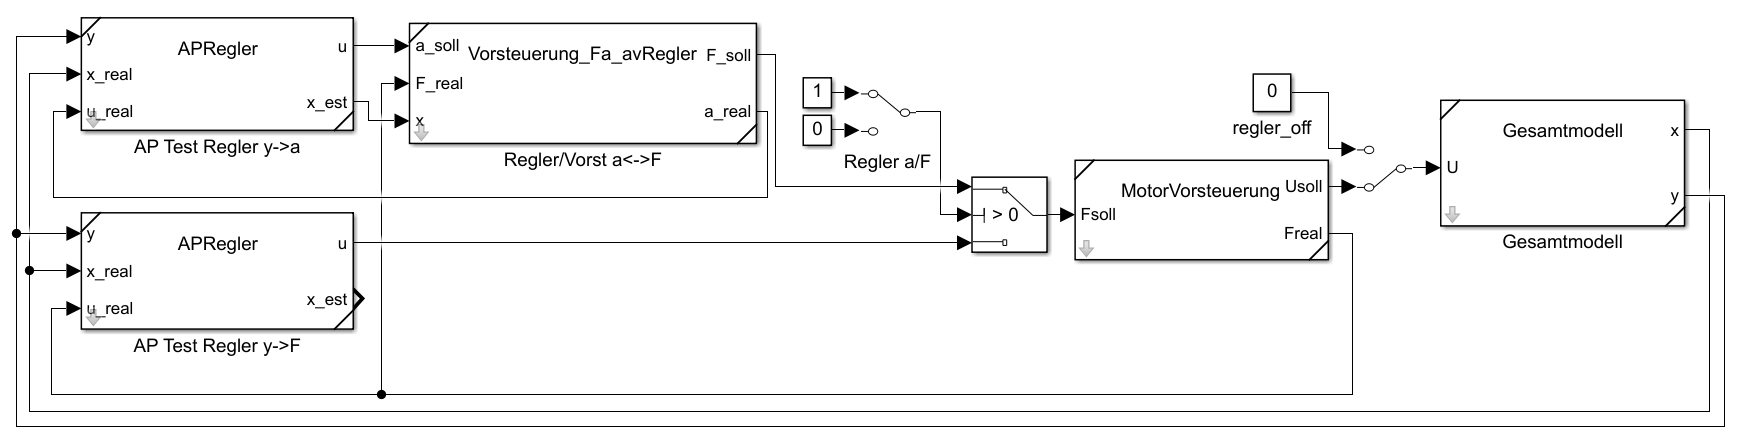
\includegraphics[width=1.00\textwidth]{Bilder/Simulink/ap_regelung_test ohne outofc.PNG}
	\caption{Aufbau der \ap-Regelung}
	\label{fig:simapr}
\end{figure}

\subsubsection{APRegler.slx}
Dieses Modul ist eine Art \qq{Wrapper} für den eigentlich \zsr, um die \ap-Transformation durchzuführen.
Erwartet als Parameter die Daten zum \ap.

\subsubsection{Zustandsregler.slx}
Implementiert einen gewöhnlichen \zsr, bei dem alle Arten der \ze\ \siehe{\secref{subsec:zse}} möglich sind \siehe{\figref{fig:simzsr}}.
Die Auswahl wird durch ein \emph{Variant Subsystem} realisiert, das durch die Variable \texttt{simparams.Zustandsermittlung} angesteuert wird.%\siehe{\figref{fig:simzse}}.
Die Stellgröße für den \beob\ kann zwischen intern und extern umgeschaltet werden.
Benötigt als Parameter die Verstärkung \texttt{K} sowie eventuelle Daten für den \beob.

\begin{figure}[htb]
	\centering
		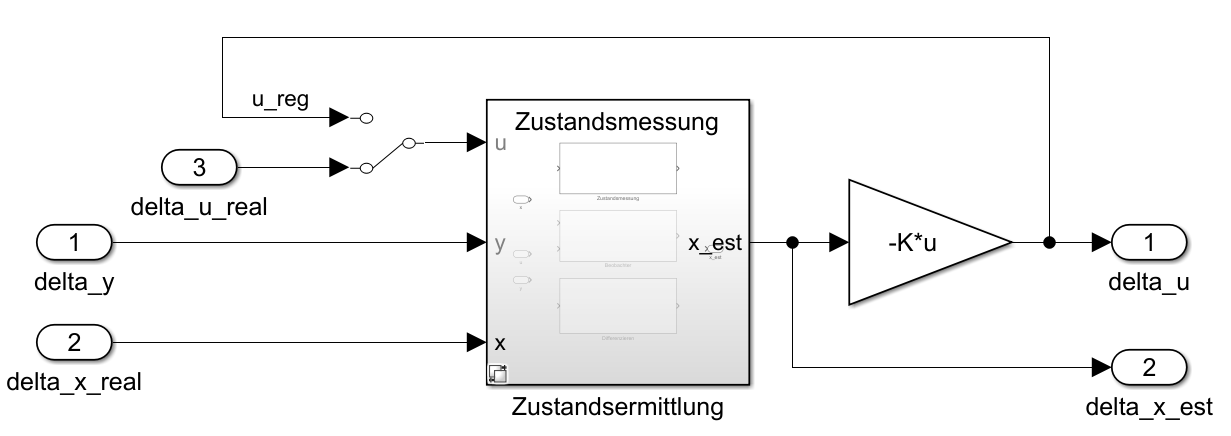
\includegraphics[width=0.8\textwidth]{Bilder/Simulink/zsr.PNG}
	\caption{\zsr\ in \sm}
	\label{fig:simzsr}
\end{figure}

%\begin{figure}[htb]
	%\centering
		%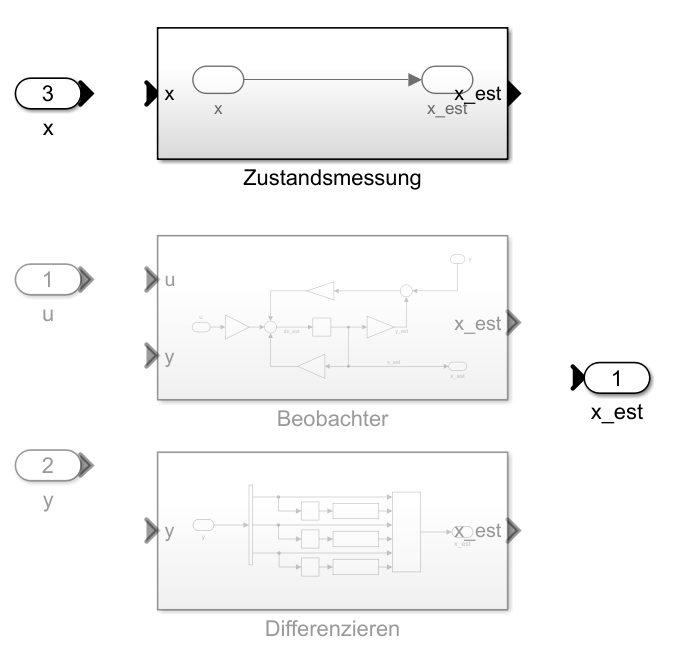
\includegraphics[width=0.35\textwidth]{Bilder/Simulink/zustandsermittlung.PNG}
	%\caption{\ze\ in \sm}
	%\label{fig:simzse}
%\end{figure}

\subsubsection{Beobachter.slx}
Implementiert einen Standard-\beob. 
Eingänge sind \texttt{u} und \texttt{y}, Ausgang sind die geschätzten Zustände \texttt{x\_est}.
Die Matrizen des linearen Systems, sowie \texttt{L} und die \beob startwerte werden über die Maske übergeben.

\subsubsection{Vorsteuerung\_Fa\_avRegler.slx}
\figref{fig:simfav} zeigt den vereinfachten Aufbau des Blocks, der die Verbindung zwischen Beschleunigung und Kraft herstellt \siehe{\secref{subsec:vorstfa}}.
Aus der Sollbeschleunigung wird mithilfe von \texttt{SchlittenGleichungKraft} die Vorsteuerkraft bestimmt.
Im Modell kann zudem zwischen dieser und der Vorsteuerungsvariante "`MCD"' (nicht dargestellt) umgeschaltet werden.
Der \avr\ wird entsprechend \secref{sec:avr} implementiert und dessen Ausgangsgröße zur Vorsteuerungskraft addiert.
Oben wird mithilfe von \texttt{SchlittenGleichungBeschleunigung} aus der nachträglich bestimmten realen Stellkraft die reale Beschleunigung berechnet.

\begin{figure}[htb]
	\centering
		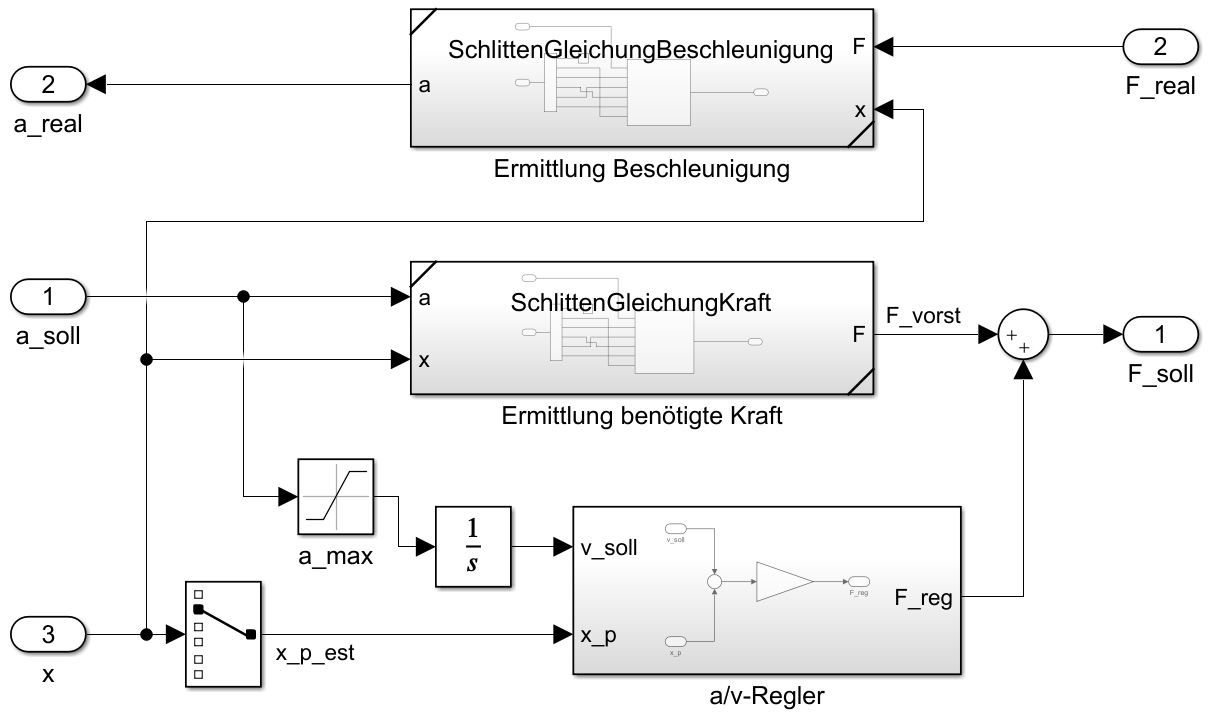
\includegraphics[width=0.7\textwidth]{Bilder/Simulink/Fa_vorst.PNG}
	\caption{Aufbau der Vorsteuerung}
	\label{fig:simfav}
\end{figure}

\subsubsection{SchlittenGleichungKraft.slx / SchlittenGleichungBeschleunigung.slx}
Setzt die Variante der Vorsteuerung mit den Systemgleichungen \siehe{\secref{sec:vorstsys}} \bzw die inverse Gleichung zur Ermittlung der Beschleunigung um.
Da diese Gleichungen symbolisch vorliegen, müssen sie mithilfe von \texttt{matlabFunctionBlock} bei der \init\ in den Block geschrieben werden.
Dadurch werden diese Dateien bei jeder \init\ oder Änderung der Systemparameter überschrieben.

\subsubsection{SchlittenVorsteuerung.slx}
Enthält die \qq{alte} Variante der Vorsteuerung \siehe{\secref{sec:vorstmcd}}.
Dabei werden die Schlittenparameter ($m_0$, \Fco\ und $d_0$) verwendet. 

\subsubsection{MotorVorsteuerung.slx}
Enthält die in \secref{sec:motvorst} beschriebene Vorsteuerung zum Motor.
Berechnet aus der Sollkraft die Sollspannung für den Motor und gibt die möglicherweise begrenzte Kraft zurück an den vorherigen Block.

\subsection{\init}

Zur \init\ der \ap-Regelung wird (nach der \init\ des Modells) das Skript \texttt{InitReg.m} ausgeführt.
Dabei werden folgende 4 Schritte durchgeführt:
\begin{enumerate}
	\item \textbf{InitSystemReg()}: Erstellt das \zrm, an dem der Regler ausgelegt wird. Dabei wird standardmäßig die beim realen System vorhandene \crb\ in den Pendelgelenken für das System des Reglers zu 0 gesetzt, um deren unverhältnismäßigen Einfluss bei der \lin\ zu vermeiden \siehe{\secref{sec:ew}}. Prinzipiell wäre es hier auch möglich, die Parameter des Reglers zu verändern, um Parameterunsicherheiten zu modellieren.
	\item \textbf{InitVorstBeob\_Fa(sysF)}: Berechnet die Vorsteuerkraft über die Systemgleichung wie in \secref{sec:vorstsys} beschrieben. Diese symbolischen Gleichungen wird mittels \texttt{matlabFunctionBlock} in die beiden entsprechenden Module geschrieben und diese werden gespeichert. 
	\item \textbf{InitAPRegData(riccdata)}: Diese Funktion berechnet die Daten für den AP-Regler anhand der gegebenen Güteparameter. Dabei werden alle \ap e linearisiert, die Reglerverstärkung mit der \ml-Funktion \texttt{lqr} und die \beob matrix berechnet.
	\item \textbf{InitSimReg(Zustandsermittlung, kpv)}: Initialisiert das Simulationsmodell für die AP-Regelung. Werte für \kpv\ und die Art der \ze\ (Standard: Messung) kann angegeben werden. Die Parameter für die Module zur Regelung werden in die \emph{struct}-Variable \path{simparams.regler} geschrieben. Die Systemparameter von Motor und \spd\ (von denen der Regler ausgeht) werden hier übergeben, da manche von ihnen für die Regelung/Vorsteuerung benötigt werden. Durch die Trennung zu den "`realen"' Werten \path{simparams.gesamtmodell} können die Parameter des Reglers grundsätzlich auch anders sein als die, mit denen das Modell simuliert wird.
\end{enumerate}



\subsection{Güteparameter (Q,R)}\label{subsec:simqr}

Ähnlich wie bei den Parametern des \spd s werden auch die Parametersätze für die \ricc-Güteparameter ausgelagert.
Diese sind für jeden \ap\ separat definiert, da jeweils andere Werte optimal sein können.
So können verschiedene Parameter einfach verglichen werden.
Vollständige Güteparameterwerte für alle \ap e fanden sich bei den Arbeiten, die sich mit der \ap-Regelung beschäftigt haben, nur in den letzten zwei.
Im Ordner \path{Regelung/Reglerparameter} befinden sich in folgenden Datensätze:
\begin{itemize}
	\item \texttt{AP\_QR\_Chang19}: Werte der Ausarbeitung von \cite{chang}
	\item \texttt{AP\_QR\_Ribeiro20}: Werte der Ausarbeitung von \cite{ribeiro}
	\item \texttt{AP\_QR\_20\_neu}: Neu bestimmte Werte, die in dieser Arbeit optimiert wurden
	\item \texttt{AP\_QR\_20\_neu\_Beob}: Neu bestimmte Werte, die in dieser Arbeit für den Einsatz mit \beob\ optimiert wurden
\end{itemize}


\subsection{Weitere \Matlab-Funktionen}

\subsubsection{SimAP}
Mit dieser Funktion wird eine Simulation mit gegebenem \ap\ und Startwerten (\ap abweichung) durchgeführt. Die Simulationszeit \texttt{Tsim} ist optional (Standard: \valunit{10}{s}).
\[
	\texttt{SimAP(testAP, delta\_x0, Tsim)}
\]
Dabei werden die Initialisierungen des \ap es, der Startwerte und der \beob startwerte vorgenommen.
Außerdem werden Auswertungen der Simulation vorgenommen \siehe{\secref{subsec:x0ausw}} und die Ergebnisse zurückgegeben.
Die Funktion kann auch mit \texttt{SimAP\_run.m} aufgerufen werden. 
Dabei werden weitere Auswertungen angezeigt, \zB die Maximalabweichungen vom \ap, ob die Stellgrößenbegrenzung aktiv war oder ob der Schlitten außerhalb der Begrenzung war.
Zusätzlich wird direkt ein Plot und eine Animation \siehe{\secref{subsec:ausw}} angezeigt.

\subsubsection{SchlittenPendelAnalyse}

Mit der Funktion \texttt{SchlittenPendelAnalyse(sys)} werden für ein gegebenes \zrm\ Eigenwerte für alle Ruhelagen berechnet und dargestellt, sowie Steuer- und Beobachtbarkeit geprüft.

\subsubsection{x0\_Tests}
Die Funktionen zu den \xots s (siehe folgender Abschnitt) und darauf aufbauenden Tests befinden sich im Ordner \path{Regelung/x0_Tests}.




\section{Anfangswert-Tests}\label{sec:x0test}

Ziel dieser Arbeit ist die "`Regelbarkeit"' des Systems zu untersuchen.
Dafür müssen zunächst Kriterien definiert werden, inwiefern das System unter festgelegten System- und Entwurfsparametern regelbar \bzw stabilisierbar ist.

Dazu wird wieder \figref{fig:regvorg} herangezogen.
Ist ein System fest ausgelegt, können die verschiedenen \ap e mit bestimmten Startwerten getestet werden.
Dabei gibt es jedoch unzählige Kombinationsmöglichkeiten, die nicht alle getestet werden können.
Es muss daher eine Auswahl an Startwerten getroffen werden.
Oft wird immer nur für einen Zustand eine Abweichung gesetzt, alle anderen sind am \ap.
Selbst dann ist es mit manuellem Testen und Ausprobieren aufwändig, ein umfassendes Bild vom Regelverhalten zu erlangen.
Die Optimierung der "`äußeren Schleifen"' wird somit langwierig und ist auf diese Weise nicht zielführend.

Daher wird die "`untere Schleife"' automatisiert.
Wird ein \ap-Test durchgeführt, können die Simulationsdaten ausgewertet werden und gewisse Gütemaße und Performance-Indikatoren bestimmt werden, um die Regelgüte zu beschreiben.
Im Vordergrund steht aber meist die Stabilität und damit die Frage, bei welchen Werten diese nicht mehr vorhanden ist.


\subsection{Auswertung eines \ap-Tests}\label{subsec:x0ausw}

Wenn \texttt{SimAP} aufgerufen wird, werden neben den Simulationsdaten auch die Ergebnisse von \path{Auswertung/AP/APAuswertung} zurückgegeben.
Dort werden \ua folgende Gütemaße, die an das übliche quadratische \ricc-Gütemaß angelehnt sind, berechnet:
\begin{subequations} \begin{align} 
	J_x &= \int_{0}^{\tend} \dvex^\transp(t) \, \mat{Q} \, \dvex(t)  \, \ud t = \int_{0}^{\tend} \Delta x_\mrm{norm}(t)  \, \ud t  \\
	J_{x,\mrm{est}} &= \int_{0}^{\tend} \left(\dvex(t)-\dvexest(t)\right)^\transp  \,\mat{Q}  \, \left(\dvex(t)-\dvexest(t)\right)  \, \ud t  \\
	J_u &= \int_{0}^{\tend}  R \cdot \Delta u(t)^2 \, \ud t	\\
	J_F &= \int_{0}^{\tend}  R \cdot F(t)^2 \, \ud t
\end{align} \end{subequations}
mit
\begin{align*}
	\mat{Q} &= \diag{25, 1, 50, 1, 50, 1 } \\
	R &= 1 
\end{align*}
Dabei beschreibt $J_x$ den kumulierten Verlauf aller Zustände als skalare Größe.
$J_{x,\mrm{est}}$ berechnet ein Maß zur Bewertung des \beob fehlers.
Die anderen beiden Maße beschreiben die kumulierte Stellgröße/-energie, hier ist $J_F$ aussagekräftiger, da es die reale Motorkraft verwendet.
Für die Berechnung werden die transformierten \ap-Zustände \dvex(t) \eqref{eq:aptransf} verwendet, da diese die Abweichung von der Ruhelage darstellen.
In \ml\ werden die Maße als Summe berechnet (der Einfachheit halber konstante Schrittweite vorausgesetzt).

Für die Beurteilung der Stabilität, also ob der Zustand am Ende der Simulationszeit noch in der Nähe des \ap es ist, wird
$\Delta x_\mrm{norm}(\tend)$
verwendet. Ist dieser skalare Wert unter einer festgelegten Schranke, wird von einer Stabilisierung des \ap es ausgegangen.

Außerdem wird für jeden Zustand die Maximalabweichung vom \ap\ bestimmt, da diese ein wichtiges Gütekriterium ist, insbesondere die Schlittenposition, da diese Beschränkungen unterliegt \siehe{\secref{sec:schlbes}}.

Des Weiteren kann anhand von $\Delta x_\mrm{norm}(t)$ eine Einschwingzeit bestimmt werden.
Diese ist dort, wo der Norm-Verlauf eine gewisse Schranke nicht mehr überschreitet.


\subsection{\xots}\label{subsec:awts}

Die Funktion \texttt{x0\_Test.m} stellt die Basis für einen Anfangswerttest dar.
Für den angegebenen \ap\ ermittelt sie mit einzelnen Simulationen und steigenden Anfangsauslenkungen vom \ap\ schrittweise die maximalen Startwerte.
Dabei wird mit obigen Methoden ermittelt, ob die Stabilisierung erfolgreich war.
Falls nicht, wird abgebrochen und der Maximalwert sowie einige der Gütemaße für allen Einzelergebnisse zurückgegeben.

Die Schrittweite \texttt{y\_st} = [ \texttt{x\_st} \texttt{phi1\_st} \texttt{phi2\_st} ] gibt die Schrittweite an, mit der die Tests ausgeführt werden.
Eine kleinere Schrittweite löst zwar die Ergebnisse besser auf, führt aber zu einer höheren Rechenzeit.

\begin{figure}[hb]
	\centering
		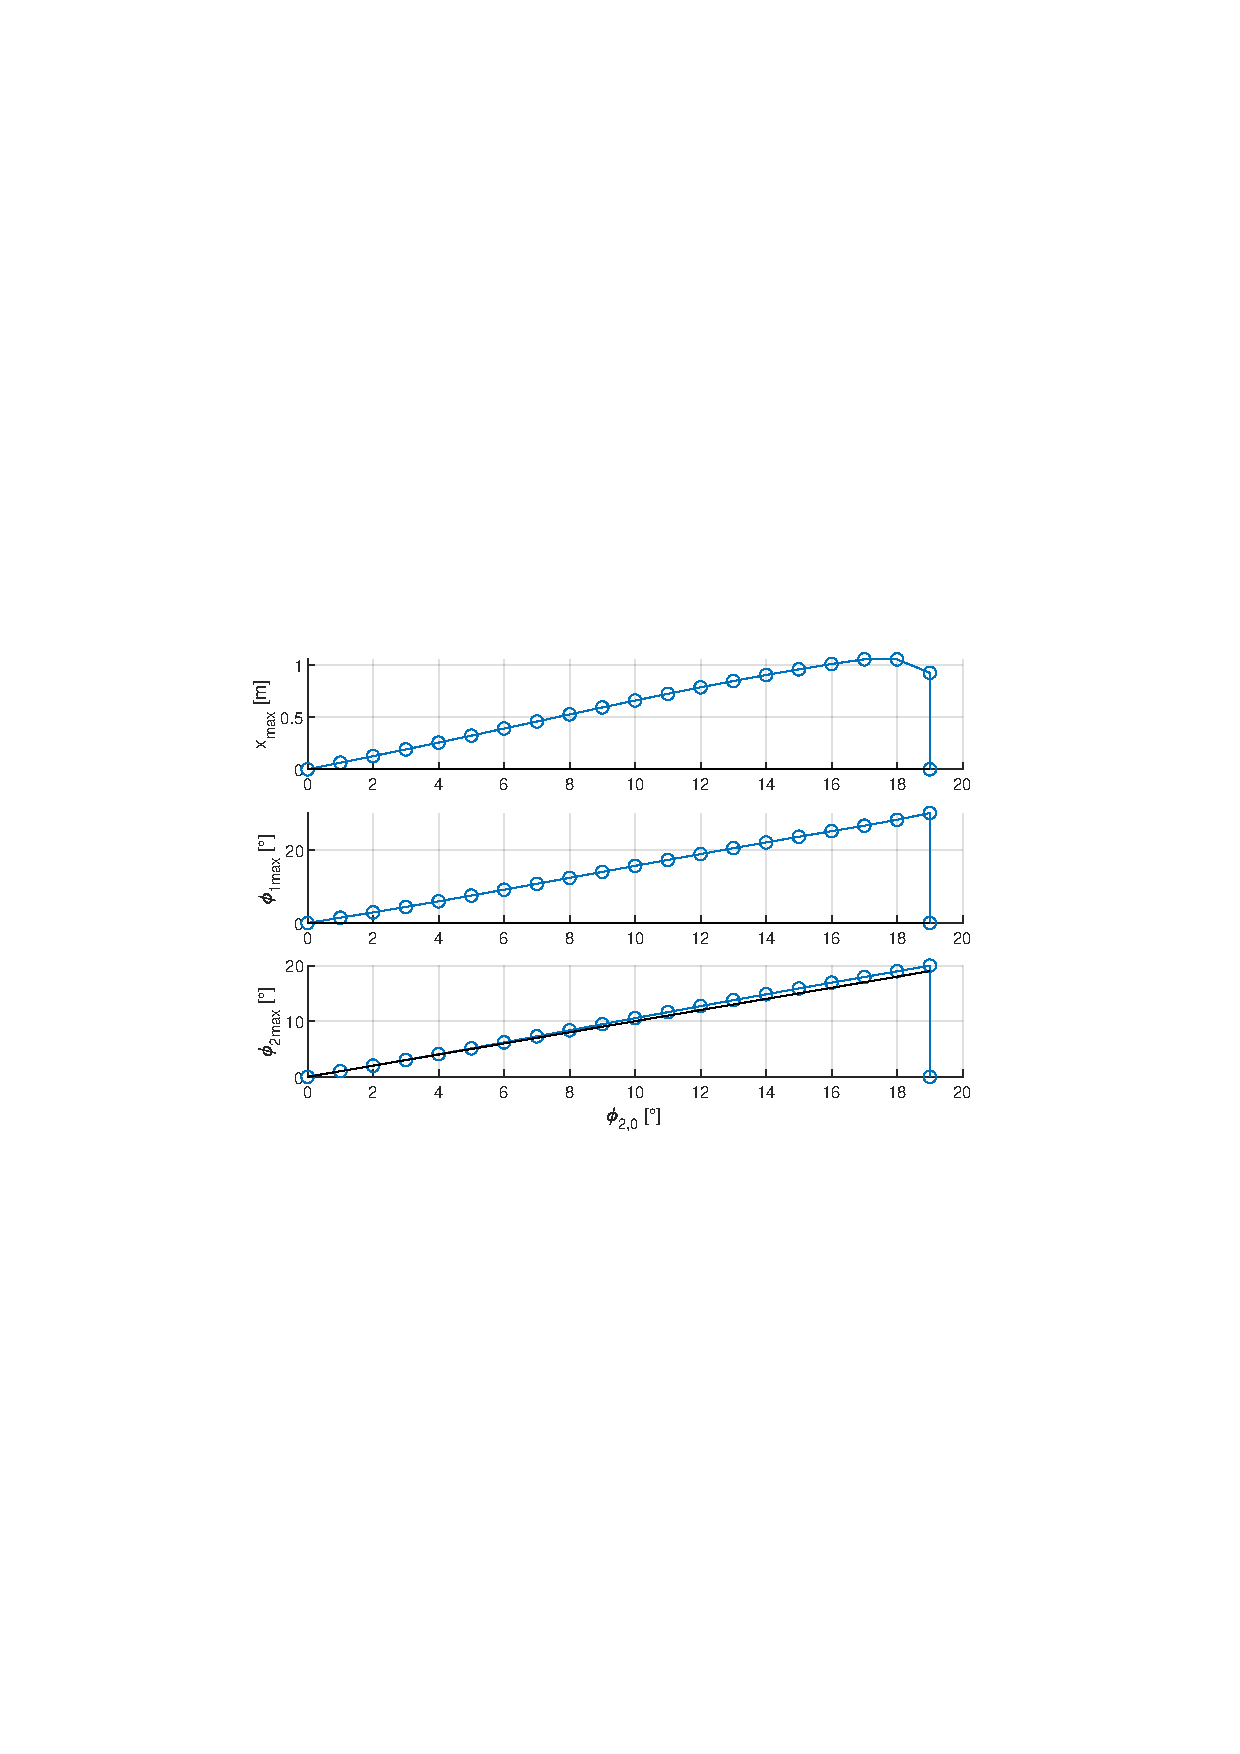
\includegraphics[width=0.75\textwidth]{Bilder/x0test/appr-x0-ap42.pdf}
	\caption{Anfangswerttest \apv, Auslenkung \phz}
	\label{fig:x0test}
\end{figure}

Die Ergebnisse eines \xots s an \apv\ sind beispielhaft in \figref{fig:x0test} dargestellt.
Auf der Abszisse wird der Startwert der Auslenkung (hier \phz) aufgetragen.
In Abhängigkeit von dieser werden die sich in der Folge ergebenden maximalen Abweichungen der drei Ausgänge vom \ap\ dargestellt.
In diesem Fall kann das System bis zu einem Startwert von $\phzo=\valdeg{19}$ stabilisiert werden.
Die Startauslenkung wird auch als schwarze Linie eingezeichnet. 
Die Maximalabweichung ist stets oberhalb oder auf dieser.


\subsection{Kritische \xots s}\label{subsec:xotskrit}

Wenn immer nur ein Zustand ausgelenkt wird, ergeben sich pro \ap\ 3 Tests, also insgesamt 9 Tests (unter Vernachlässigung des stabilen \ape).
Es hat sich dabei gezeigt, dass Abweichungen von \xo\ kein Problem bezüglich der Stabilität darstellen.
Außerdem sind bei \ap\ 2 und 3 Auslenkungen des jeweils "`stabilen"' Pendels unkritisch.

Aus diesem Grund sind für die Untersuchung der Stabilität nur die folgenden vier (kritischen) Anfangswert-Tests relevant:
\begin{itemize}
	\item \texttt{\apz}: \ap\ 2, Auslenkung \phz
	\item \texttt{\apd}: \ap\ 3, Auslenkung \phe
	\item \texttt{\apv 1}: \ap\ 4, Auslenkung \phe
	\item \texttt{\apv 2}: \ap\ 4, Auslenkung \phz
\end{itemize}
In \texttt{x0\_Test\_APs.m} werden diese vier Tests durchgeführt und die Ergebnisse zur weiteren Darstellung gespeichert.
Maßgeblicher Indikator für die Stabilität ist die jeweilige maximale Auslenkung \phe\ oder \phz, bis zur welcher das System noch stabilisiert werden kann.

Diese Tests können nun mit verschiedenen Systemen durchgeführt werden und miteinander verglichen werden.
Dabei können Regelparameter oder auch Systemparameter variiert werden.
Der Vorteil dieser Darstellung ist, dass die Gütekriterien wie Maximalabweichungen, die obigen Gütemaße und die Einschwingzeit direkt im selben Diagramm für alle Startwerte verglichen werden können.
Dadurch lässt sich die Güte der Regelung \bzw die Regelbarkeit einer Konfiguration auf einen Blick beurteilen.



\newcommand{\scalee}{0.48}
\begin{figure}[htbp]
	\centering
	\subfloat[\apaz]{ 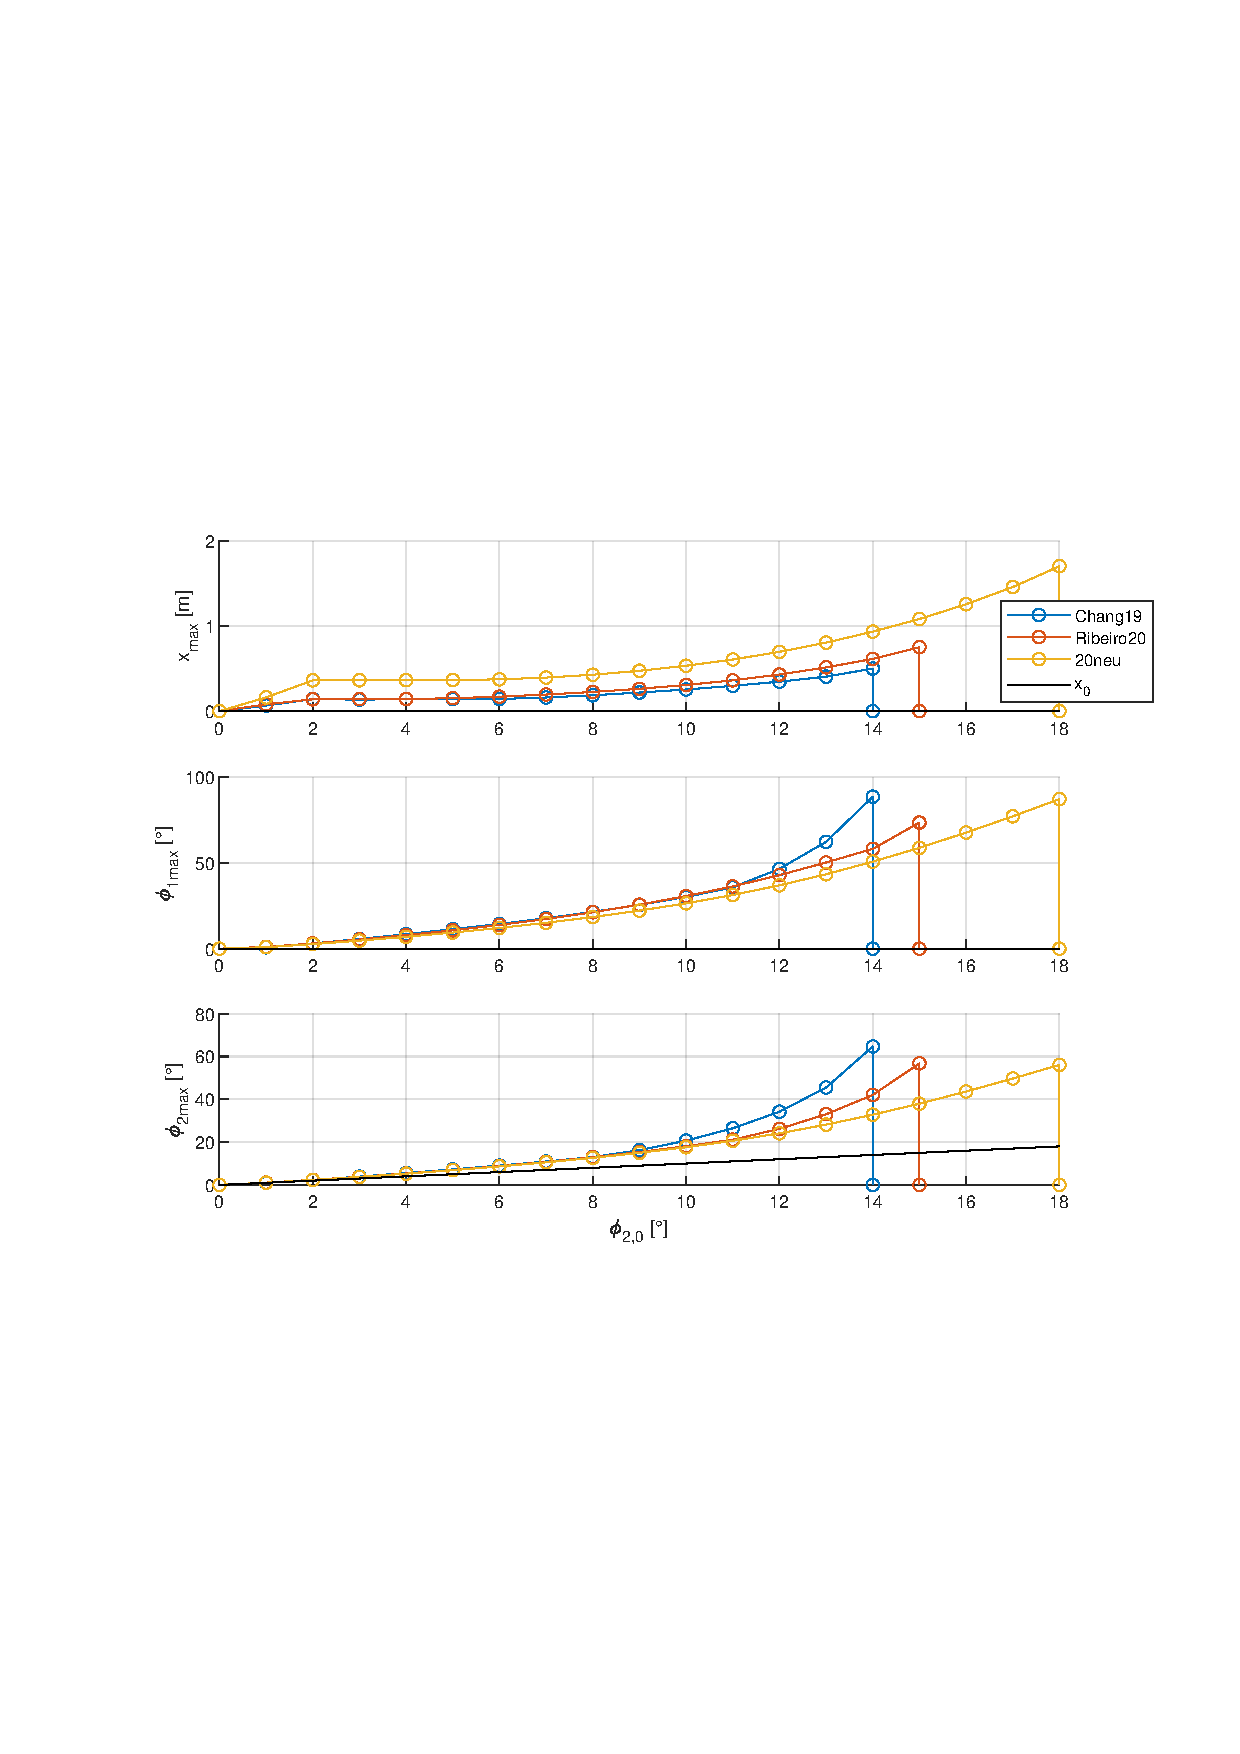
\includegraphics[scale=\scalee]{Bilder/x0QRparamVergleich/Parameter neu (Ribeiro) Creg off/AP2.pdf} }
	\hfil
	\subfloat[\apad]{	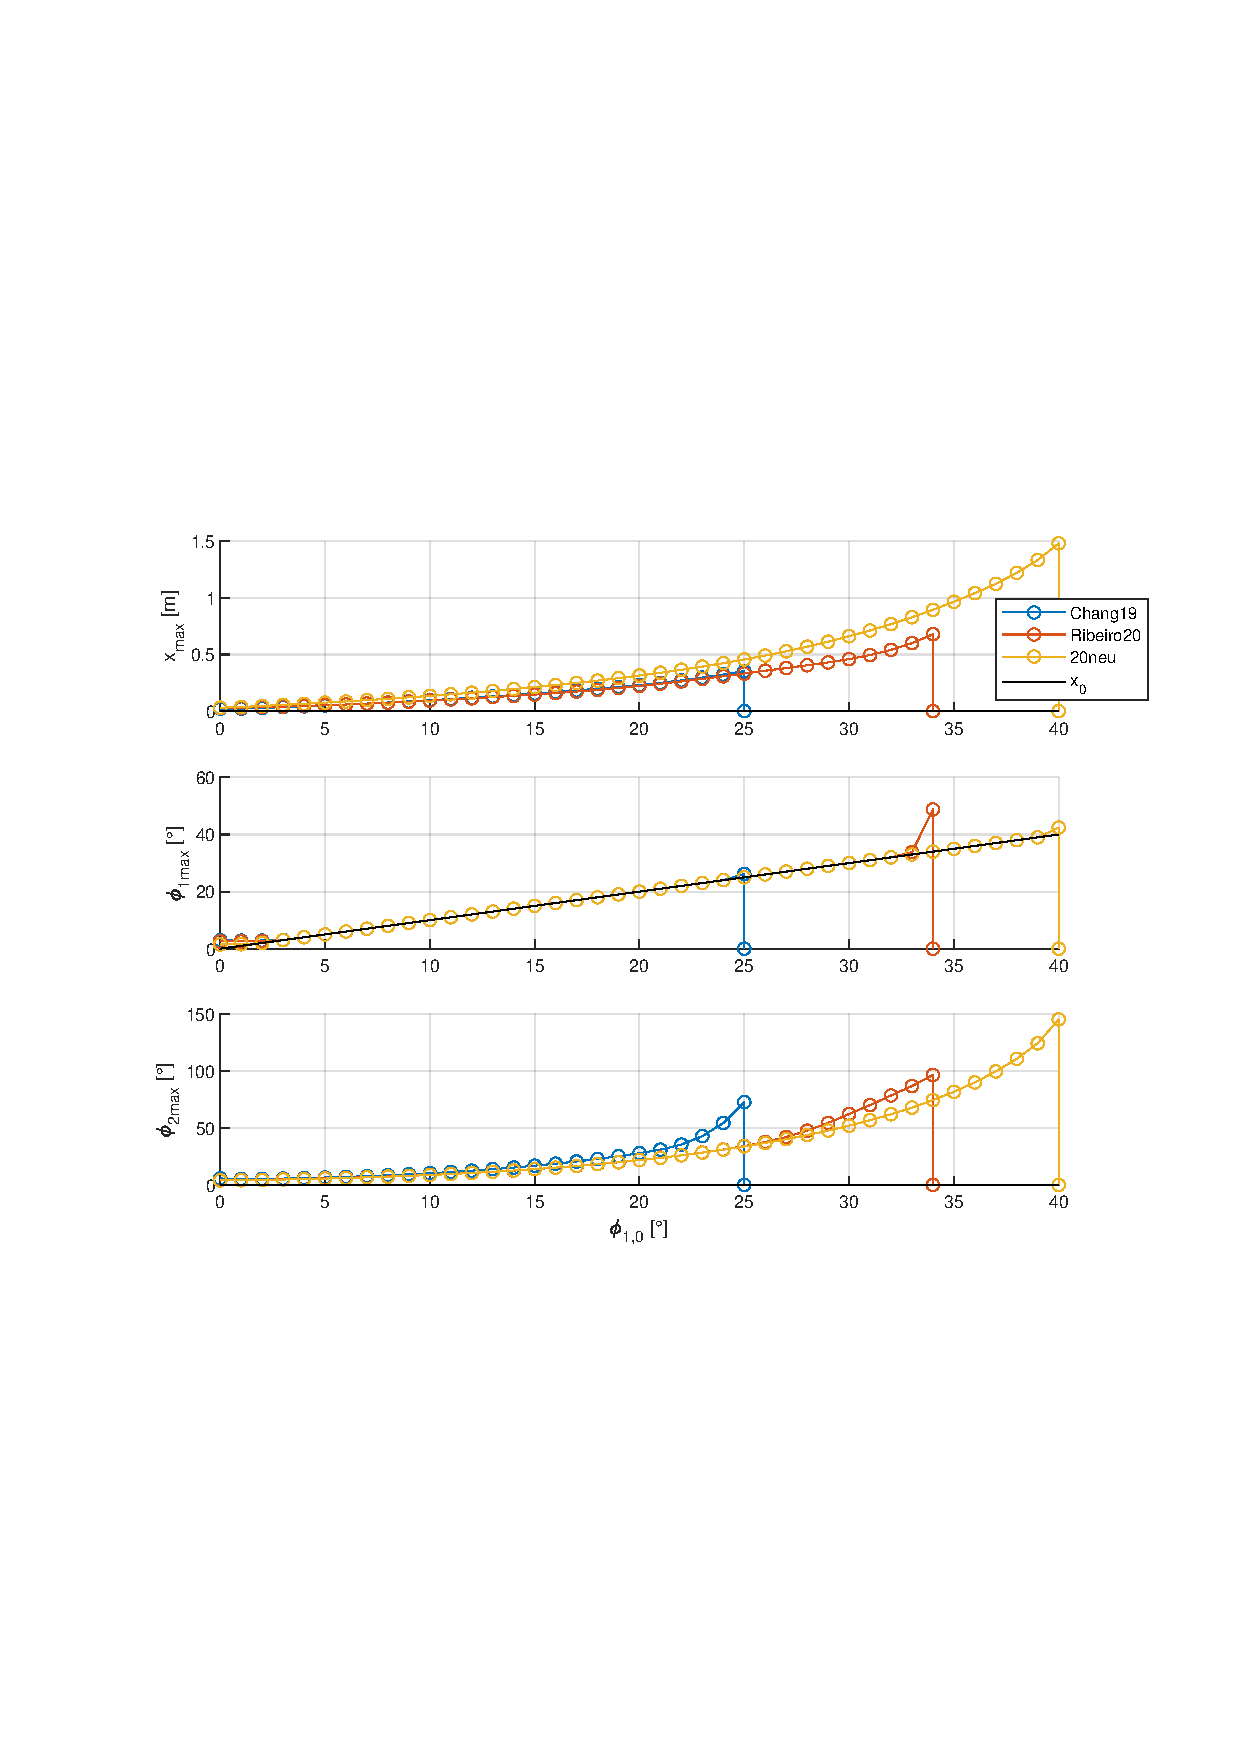
\includegraphics[scale=\scalee]{Bilder/x0QRparamVergleich/Parameter neu (Ribeiro) Creg off/AP3.pdf} }
	\\
	\subfloat[\apave]{ 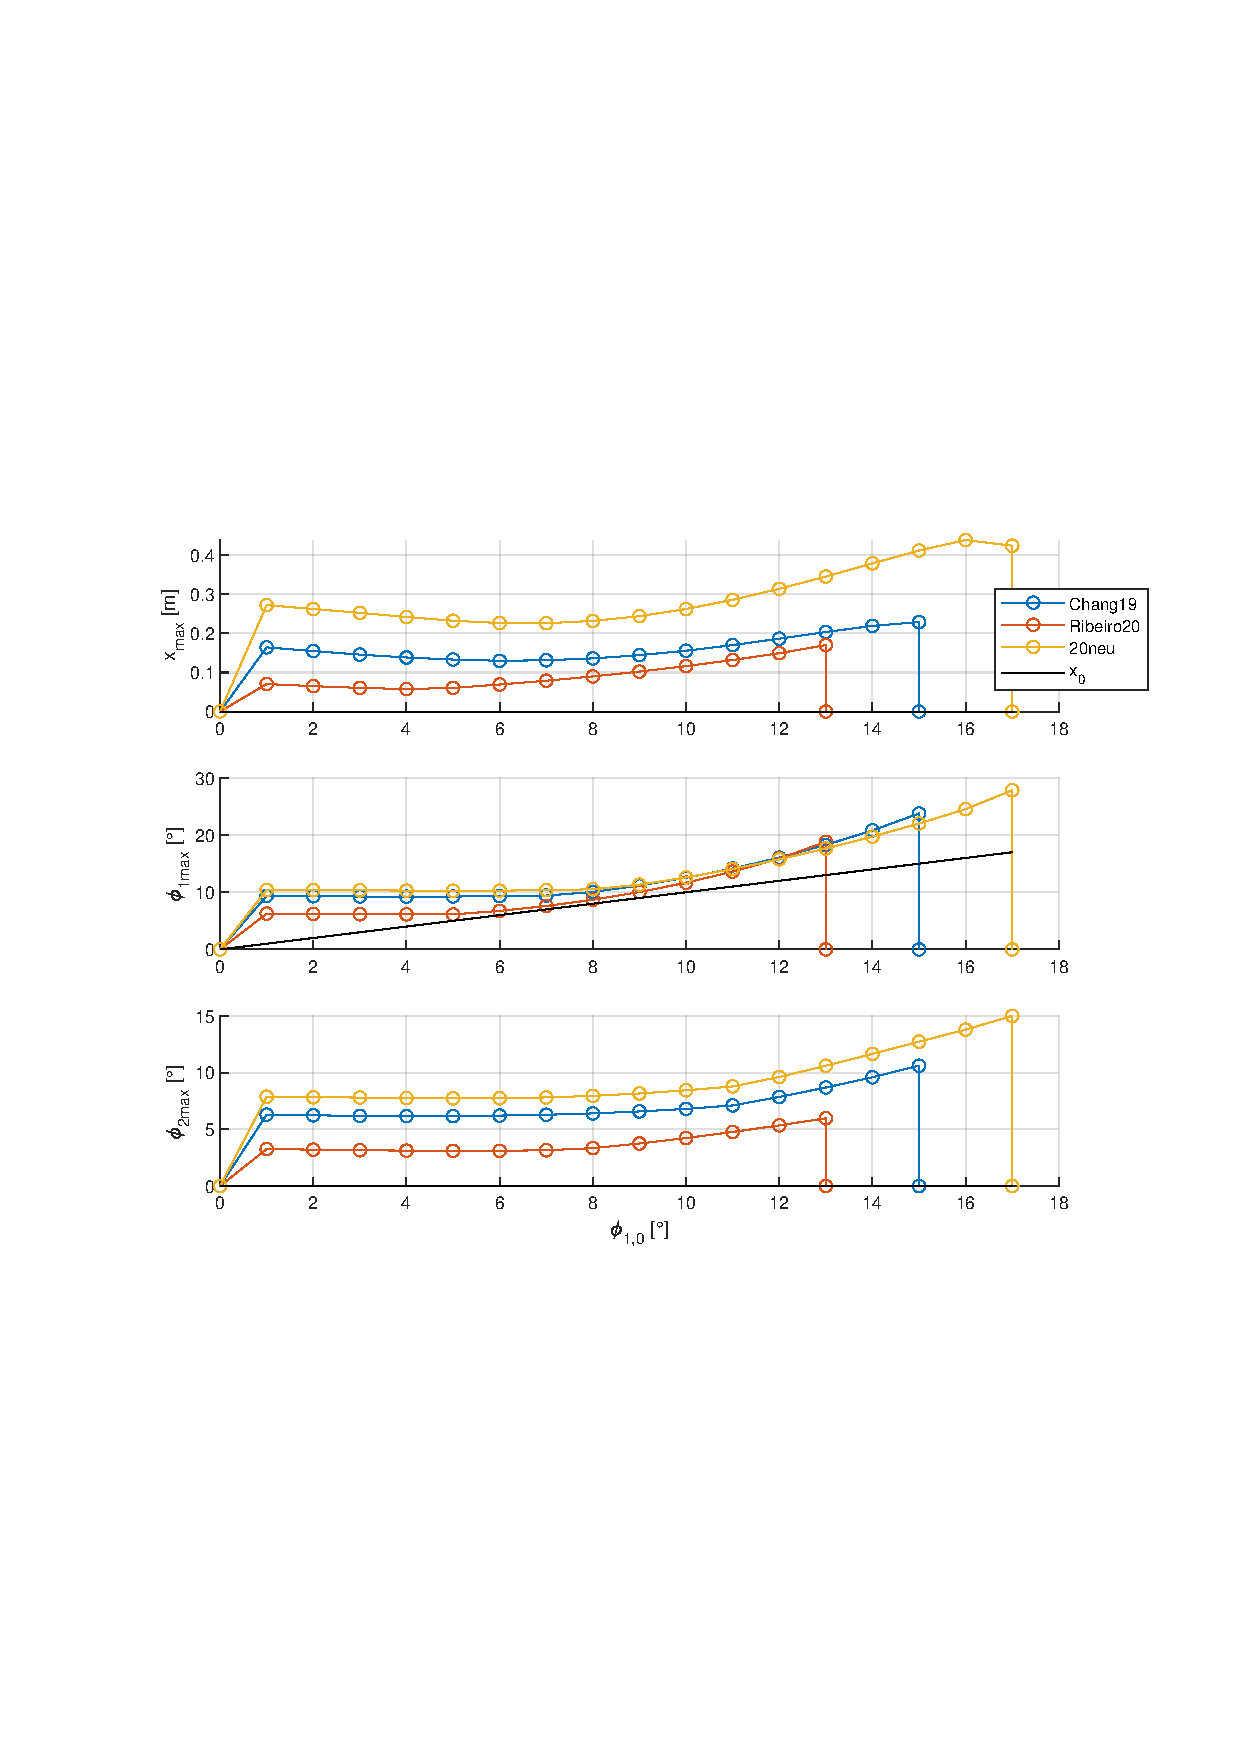
\includegraphics[scale=\scalee]{Bilder/x0QRparamVergleich/Parameter neu (Ribeiro) Creg off/AP41.pdf} }
	\hfil
	\subfloat[\apavz]{ 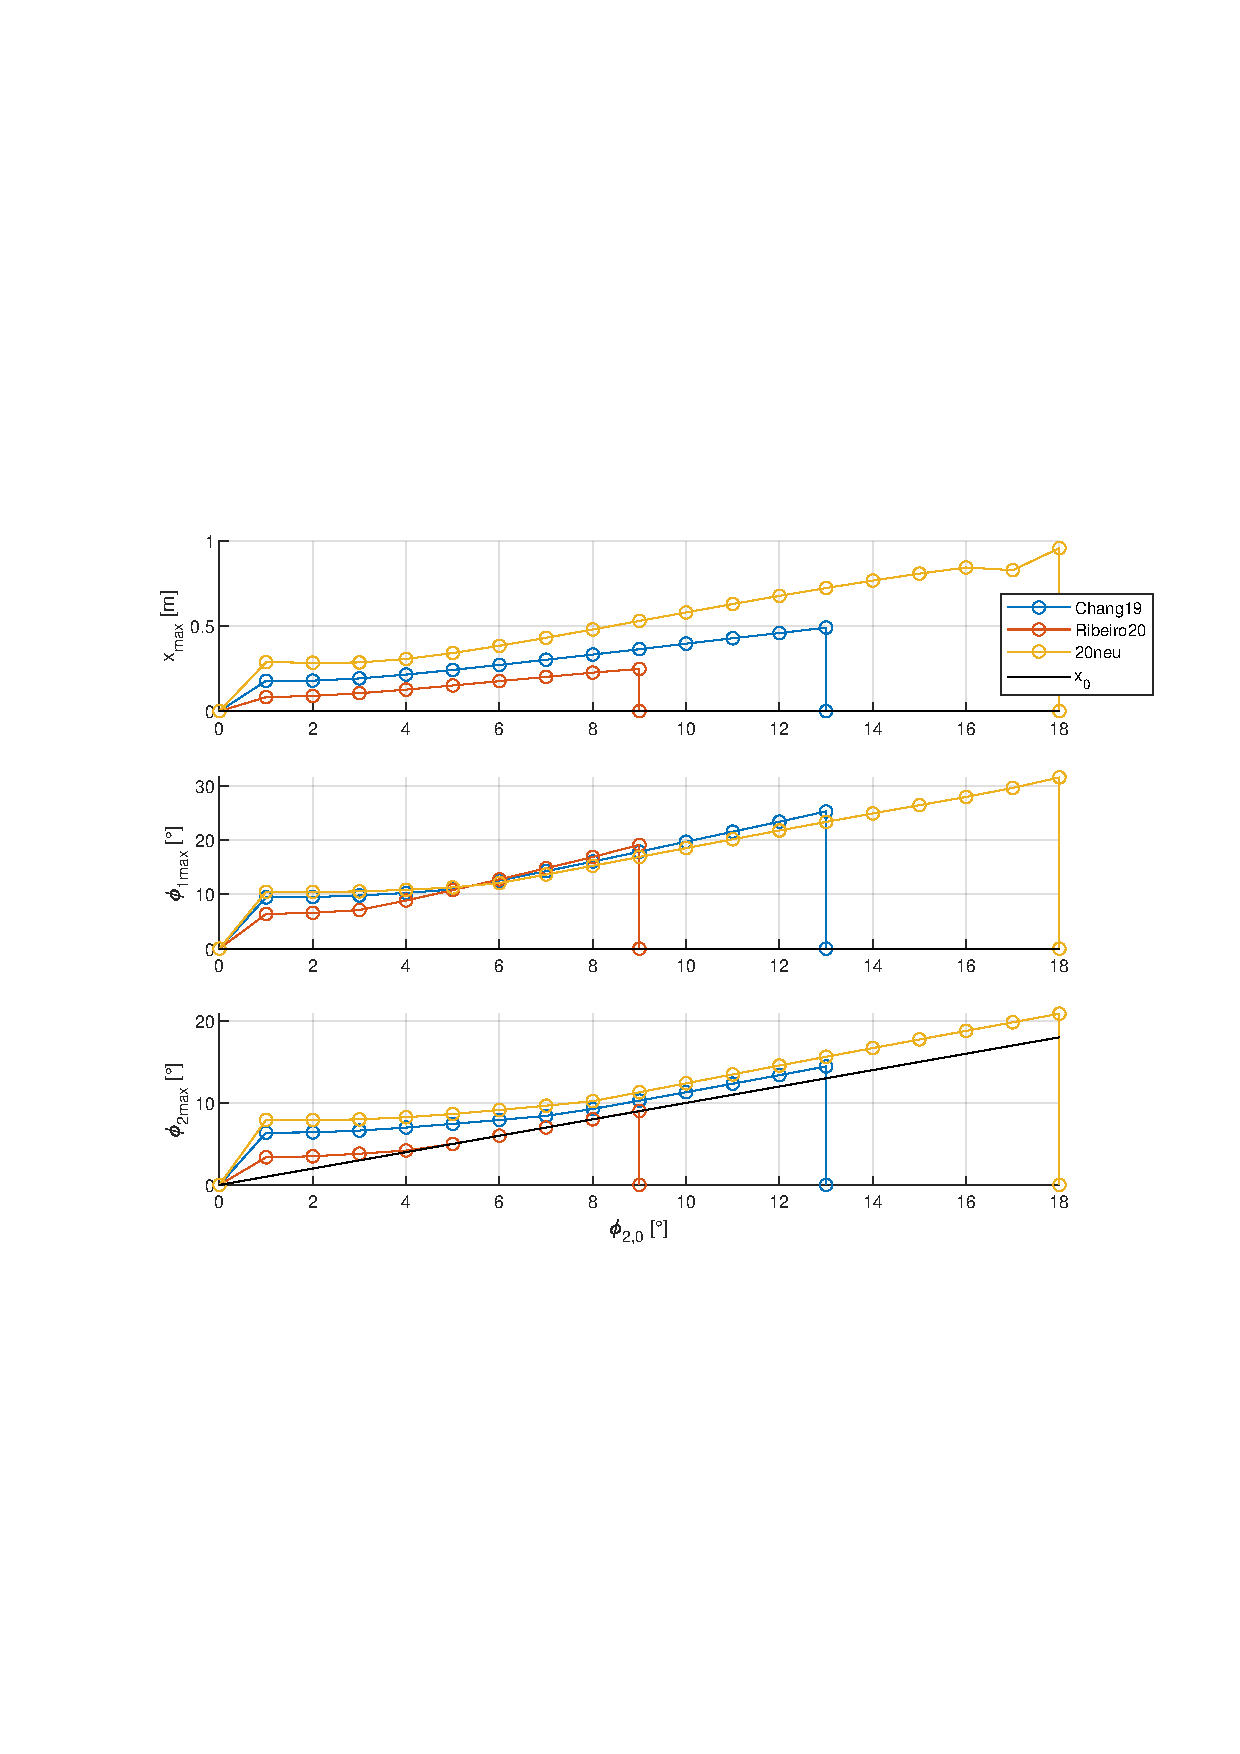
\includegraphics[scale=\scalee]{Bilder/x0QRparamVergleich/Parameter neu (Ribeiro) Creg off/AP42.pdf} }
	\caption{Maximalabweichungen -- Vergleich QR-Parameter (System Ribeiro)}
	\label{fig:qrvglrib}
\end{figure}

\subsection{Vergleiche von \xots s}\label{subsec:xotsvgl}

Beispielsweise kann man die Ergebnisse mit verschiedenen \ricc-Parametern \mat{Q} und $R$ vergleichen.
In \figref{fig:qrvglrib} sind die Maximalabweichungen mit den verschiedenen QR-Parametern \siehe{\secref{subsec:simqr}} am neuen System dargestellt.
Die Wahl der QR-Parameter hat offenbar einen wichtigen Einfluss auf Stabilisierbarkeit und Regelgüte.
Insgesamt lässt sich feststellen, dass \apd\ die größten Startabweichungen ausregeln kann.
Die in dieser Arbeit optimierten Parameter können das \dpd\ bei allen \ap en in einem etwas größeren Bereich stabilisieren.
Allerdings sieht man auch \zB an \apve, dass das meist auf Kosten höherer Abweichungen bei den niedrigeren Startwerten geschieht.
Bei den Reglerparametern ist somit immer ein gewisser Kompromiss notwendig.


Bei der Regelung mit den neuen Pendelparametern \texttt{Ribeiro20} ist im Vergleich zu den alten Parametern \texttt{Apprich09} aufgefallen, dass der Endwert nicht mehr asymptotisch erreicht wird, sondern sich ein Grenzzyklus einstellt.
Die Ursache dafür liegt sehr wahrscheinlich in der \crb\ der Pendelgelenke \siehe{\tabref{tab:spdparams}}, die beim alten System nicht vorhanden ist.

\renewcommand{\scalee}{0.53}
\begin{figure}[htbp]
	\centering
	\subfloat[\apaz]{ \includegraphics[scale=\scalee]{Bilder/x0QRparamVergleich/Parameter alt+neu/AP2.pdf} }
	%\hfil
	\subfloat[\apad]{	\includegraphics[scale=\scalee]{Bilder/x0QRparamVergleich/Parameter alt+neu/AP3.pdf} }
	\\
	\subfloat[\apave]{ \includegraphics[scale=\scalee]{Bilder/x0QRparamVergleich/Parameter alt+neu/AP41.pdf} }
	%\hfil
	\subfloat[\apavz]{ \includegraphics[scale=\scalee]{Bilder/x0QRparamVergleich/Parameter alt+neu/AP42.pdf} }
	\caption{Maximalabweichungen -- Vergleich alter und neuer Pendelparameter}
	\label{fig:vglpendelpar}
\end{figure}

\figref{fig:vglpendelpar} vergleicht die beiden Systeme, sowie eine Variante, bei der die \crb smomente zu 0 gesetzt werden (\texttt{MCoff}).
Bei allen \ap en fällt auf, dass das System mit den \crb smomenten bei sehr niedrigen Startwerten höhere Maximalabweichungen zeigt, die durch die Dauerschwingung verursacht werden.
\ZB ergibt sich bei \apz\ ab einem Startwert von $\pheo=\valdeg{2}$ ein Positionssausschlag von \valunit{0,3}{m}.
Bei \apd\ und \apv\ ergibt sich sogar bei einem Startwert von 0 eine Dauerschwingung (was bei \apd\ auf die numerische Ungenauigkeit von $\pi$ zurückzuführen ist, bei \apv\ erst mit einer minimalen Anregung).
Da die Maximalabweichungen insbesondere bei \apv\ über einen weiten Bereich konstant sind ($\phem=\valdeg{10}$, $\phzm=\valdeg{8}$), besteht die Vermutung, dass der Grenzzyklus fast unabhängig von den Startwerten ist.
Die alten Parameter sowie die neuen Parameter mit ausgeschalteter \crb\ in den Gelenken zeigen dieses Verhalten nicht und beginnen in 0 mit einem etwa linearen Verlauf.
Aus diesem Grund wird die nichtlineare \crb\ als Ursache dafür gesehen.


\renewcommand{\scalee}{0.62}
\begin{figure}[htbp]
	\centering
	\subfloat[\apaz]{ \includegraphics[scale=\scalee]{Bilder/x0QRparamVergleich/Parameter neu (Ribeiro) ZM+Beob/AP2.pdf} }
	\hfil
	\subfloat[\apad]{	\includegraphics[scale=\scalee]{Bilder/x0QRparamVergleich/Parameter neu (Ribeiro) ZM+Beob/AP3.pdf} }
	\\
	\subfloat[\apave]{ \includegraphics[scale=\scalee]{Bilder/x0QRparamVergleich/Parameter neu (Ribeiro) ZM+Beob/AP41.pdf} }
	\hfil
	\subfloat[\apavz]{ \includegraphics[scale=\scalee]{Bilder/x0QRparamVergleich/Parameter neu (Ribeiro) ZM+Beob/AP42.pdf} }
	\caption{Maximalabweichungen -- Vergleich \zm/\beob\ (System Ribeiro)}
	\label{fig:vglribze}
\end{figure}

Auch der Einfluss des \beob\ lässt sich mit den kritischen \xots s gut darstellen.
Beim Test des \beob s an der Neukonstruktion ist zunächst aufgefallen, dass die QR-Parameter, die vorher für die Zustandsmessung optimiert wurden, nur bei \apz\ brauchbare Ergebnisse zeigten.
Bei \apv\ versagten zudem die beiden Vergleichsparameter der letzten Arbeiten.
Aus diesem Grund wurde ein neuer QR-Datensatz erstellt \siehe{\secref{subsec:simqr}}, der speziell für die Regelung mit \beob\ optimiert ist.

\figref{fig:vglribze} vergleicht daher die \ap-Regelung mit \zm\ (ZM) und \beob\ (Beob), einerseits mit den QR-Parametern \texttt{AP\_QR\_20\_neu}, sowie mit den angepassten QR-Parametern \texttt{AP\_QR\_20\_neu\_Beob} (Beob (neu)).
Während bei \apz\ und \apd\ (nur die \beob-QR-Werte) die Regler-Performance vergleichbar ist, zeigt sich bei \apv, dass der \beob\ das System nicht so weit stabilisieren kann wie mit der \zm. 
Die maximalen Startwerte sind mit $\varphi_{1,0\mrm{max}}=\valdeg{14}$ und $\varphi_{2,0\mrm{max}}=\valdeg{10}$ niedriger, außerdem sind die Winkelausschläge höher.




\section{QR Parameter Tests}\label{sec:x0qr}

Wie schon festgestellt wurde, haben Reglerparameter nicht nur einen wesentlichen Einfluss auf die Dynamik, sondern auch auf die Stabilität und damit Regelbarkeit des Systems.
Daher ist es sinnvoll, deren Einfluss in einem nächsten Schritt zu untersuchen und diese zu optimieren \siehe{\figref{fig:regvorg}}.
Dabei werden in dieser Arbeit hauptsächlich die \ricc-Güteparameter $\mat{Q}=\diaga \left(\begin{matrix} Q_1 & Q_2 & Q_3 & Q_4 & Q_5 & Q_6 \end{matrix}\right)$ und $R$ betrachtet, da diese einen deutlichen Einfluss auf die \aprg\ haben.
Andere Reglerparameter wie \kpv\ oder die \beob pole könnten ebenfalls optimiert werden, jedoch haben diese auf den ersten Blick keinen entscheidenden Einfluss.


\subsection{Vorgehen bei der Optimierung}

Die Gütematrizen wurden in den meisten vergangenen Arbeiten und anfangs auch in dieser heuristisch bestimmt und iterativ manuell angepasst.
Dieses Vorgehen ist auf Dauer sehr aufwändig und garantiert aufgrund der vielen Variationsmöglichkeiten keinesfalls optimale Werte.
Auch muss beachtet werden, dass jede Änderung an Systemparametern oder das Umschalten zum \beob\ sehr wahrscheinlich zu anderen optimalen Werten führt.
Bei \cite{chang} wurde eine Zufallssuche zum Finden von geeigneten Reglerparametern durchgeführt.
Dort wurde aber lediglich eine feste Anfangsauslenkung von \phz\ getestet, bei der Auswertung wurde eine feste obere Schranke für die maximale Schlittenposition und Endwert der Winkel verwendet.

Durch die \xots s \siehe{\secref{subsec:awts}} kann schnell ein Bild des Regelverhaltens erlangt werden.
Bei den Vergleichen in \secref{subsec:xotsvgl} wurden lediglich feste QR-Parametersätze verglichen.
Zur gezielten Optimierung liegt es nahe, einzelne Parameter zu variieren und deren Auswirkungen in den Diagrammen der \xots\ zu untersuchen.
So können die einzelnen Parameter schrittweise optimiert werden, wobei selbstverständlich zu beachten ist, dass es sich eigentlich um eine multi-variable Optimierung handelt (mit 6 Freiheitsgraden) und sich daher die Ergebnisse eines Parameters nach Änderung der anderen Parameter wieder ändern können.
Durch iteratives Vorgehen können die Werte trotzdem sehr gut optimiert und das Regelverhalten deutlich verbessert werden.


\subsection{Anwendung in \ml}

Da die Güteparameter für jeden \ap\ festgelegt werden, findet die Variation der Parameter für einen festen \ap\ statt.
Des Weiteren wird der Funktion \texttt{QR\_Variation} ein QR-Datensatz und der Parameter gegeben, der zu variieren ist (\texttt{R} oder \texttt{Qi}).
Außerdem müssen die Werte angegeben werden, welche der Parameter annehmen soll.
Um die Parameter gleichmäßig über einen großen Bereich zu testen, eignet sich ein logarithmischer Bereich, wofür die \ml-Funktion \texttt{logspace} genutzt wird. Ein beispielhafter Aufruf lautet:
	\[
	\texttt{QR\_Variation(2, AP\_QR\_20\_neu(), 'Q1', logspace(-2,2,7), 2:3 )}
\]
In der Funktion sind mehr Informationen angegeben und in \texttt{QR\_Variation\_run.m} weitere Anwendungsbeispiele zum Verwenden der Parametervariation vorhanden.

Welche der Zustände für den Test mithilfe der \xots s ausgelenkt werden sollen, kann angegeben werden.
So kann man nur die jeweils "`kritischen"' Tests ausführen \siehe{\secref{subsec:xotskrit}}, aber auch die Auswirkungen bei Startwerten der anderen Zustände untersuchen und optimieren.
Auch hier ist meistens ein Kompromiss notwendig, der für einen \ap\ verschiedene Anfangswertkombinationen gut ausregelt.


\subsection{Diagramme}

\begin{figure}[htbp]
	\centering
		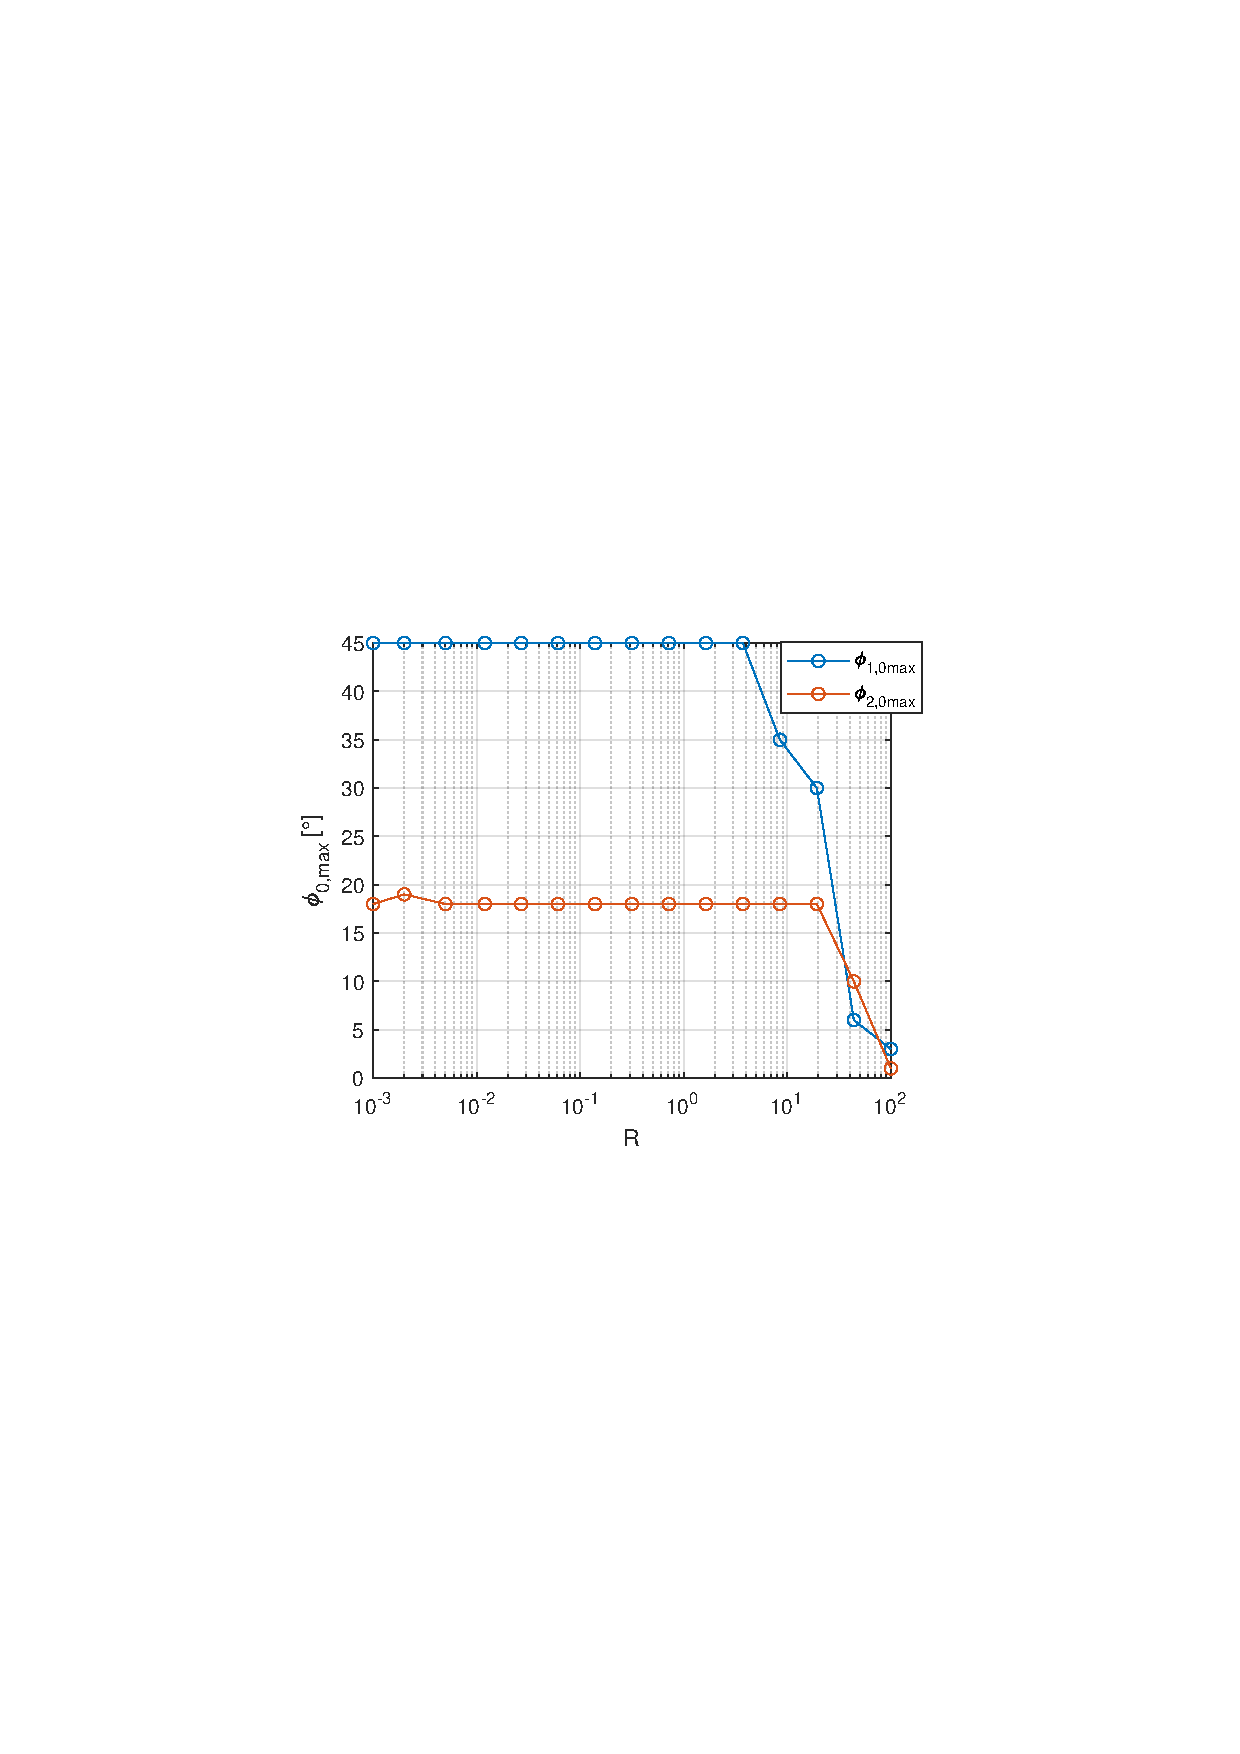
\includegraphics[width=0.55\textwidth]{Bilder/QRVariation/ap2/R phi12.pdf}
	\caption{Maximale Startwerte -- Variation von R bei \apz}
	\label{fig:qrap2R}
\end{figure}

In \figref{fig:qrap2R} werden die maximalen Startwerte von \phe\ und \phz\ bei \apz\ in Abhängigkeit von $R$ dargestellt.
Beim ersten Pendel, welches bei \apz\ stabil ist, gelingt die Stabilisierung über dem größten Bereich (ab \valdeg{45} wird der Test abgebrochen).
Die maximale Startauslenkung von \phz\ beträgt meistens \valdeg{18} und bricht ab $R=20$ ebenfalls ein.
Als Schlussfolgerung für den Parameter R gilt hier daher: je kleiner desto besser.

\begin{figure}[htbp]
	\centering
		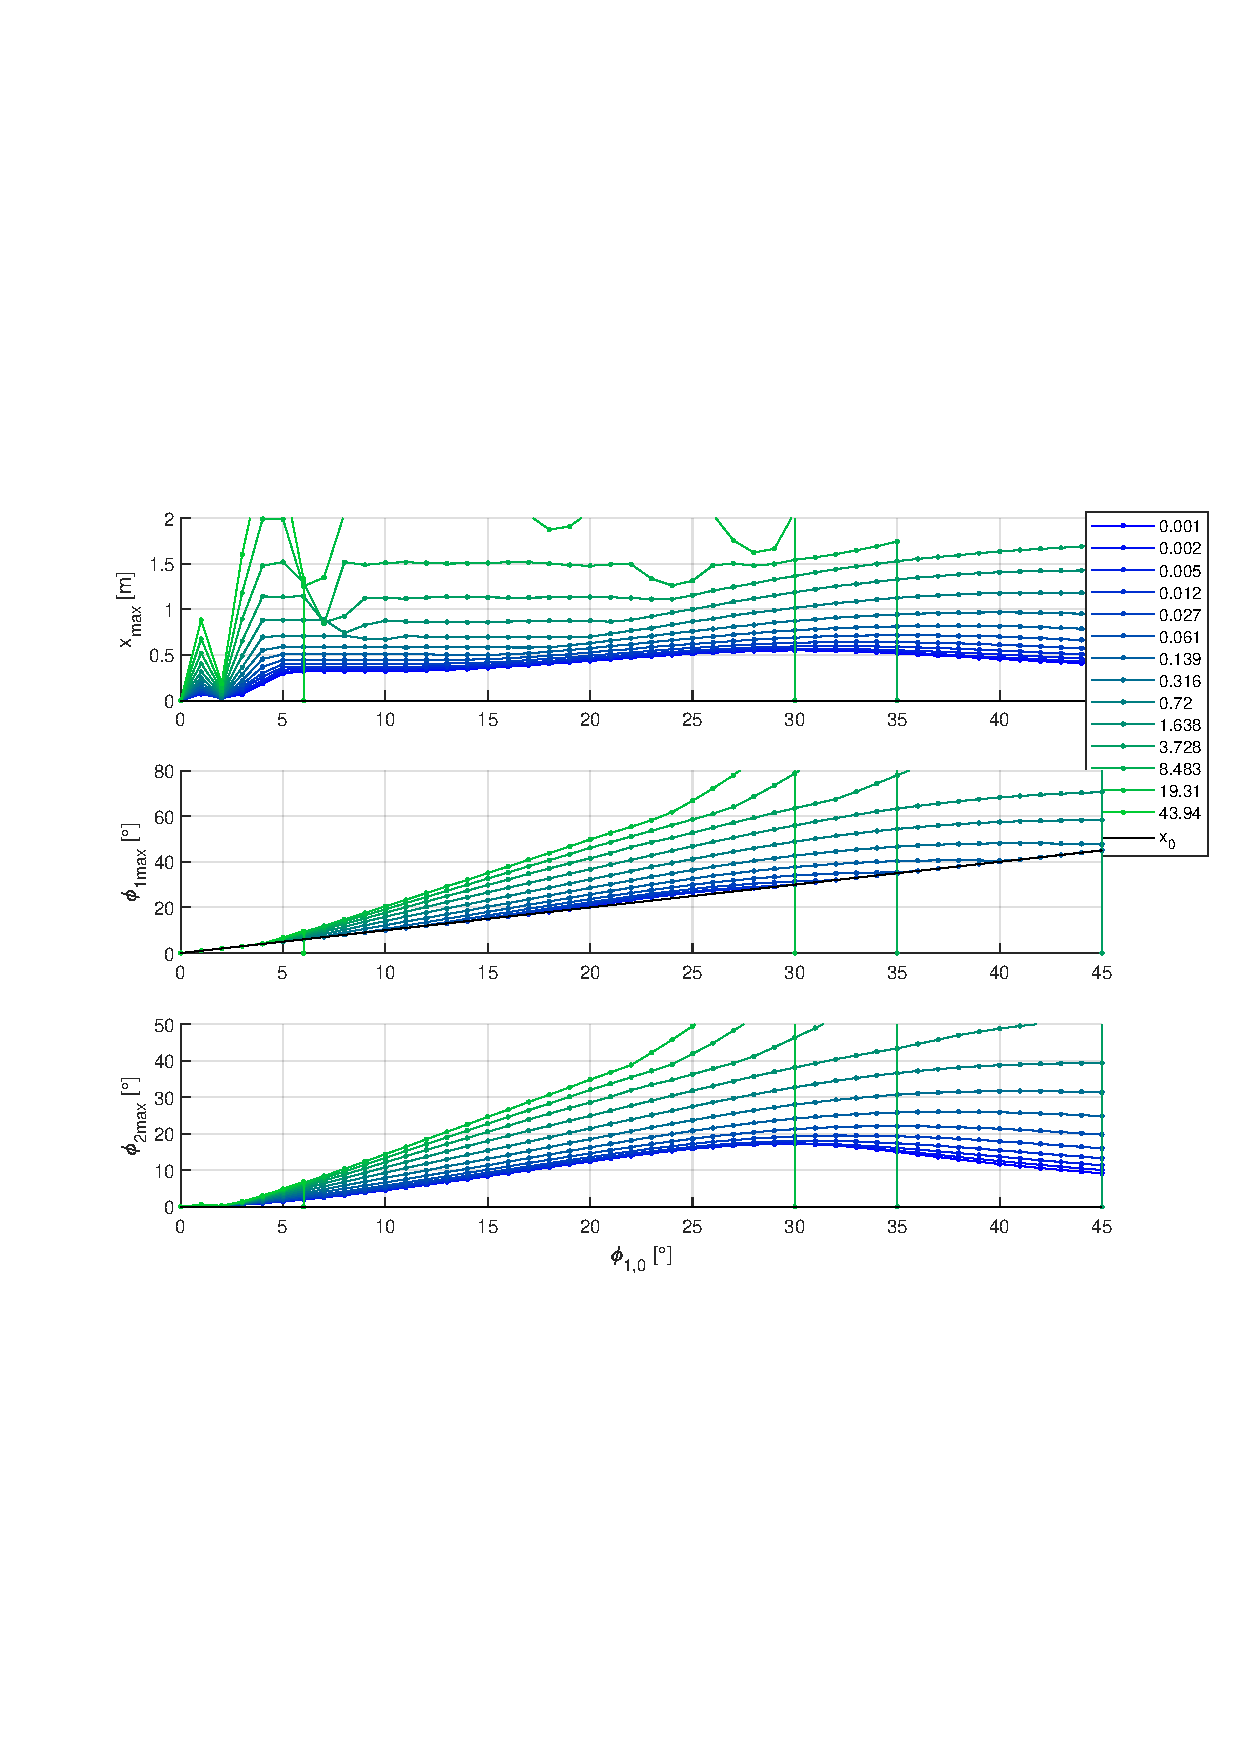
\includegraphics[width=0.9\textwidth]{Bilder/QRVariation/ap2/R phi1 m.pdf}
	\caption{Maximalabweichungen -- Variation von R bei \apz}
	\label{fig:qrap2Rm}
\end{figure}

Allerdings muss auch die Dynamik, insbesondere die resultierenden Maximalausschläge der Zustände, beachtet werden.
\figref{fig:qrap2Rm} stellt daher für dieselbe Konfiguration die Maximalabweichungen dar, bei Auslenkung von \phe.
Hier zeigt sich ebenfalls ein besseres Verhalten bei kleineren Werten von $R$.

\begin{figure}[htbp]
	\centering
		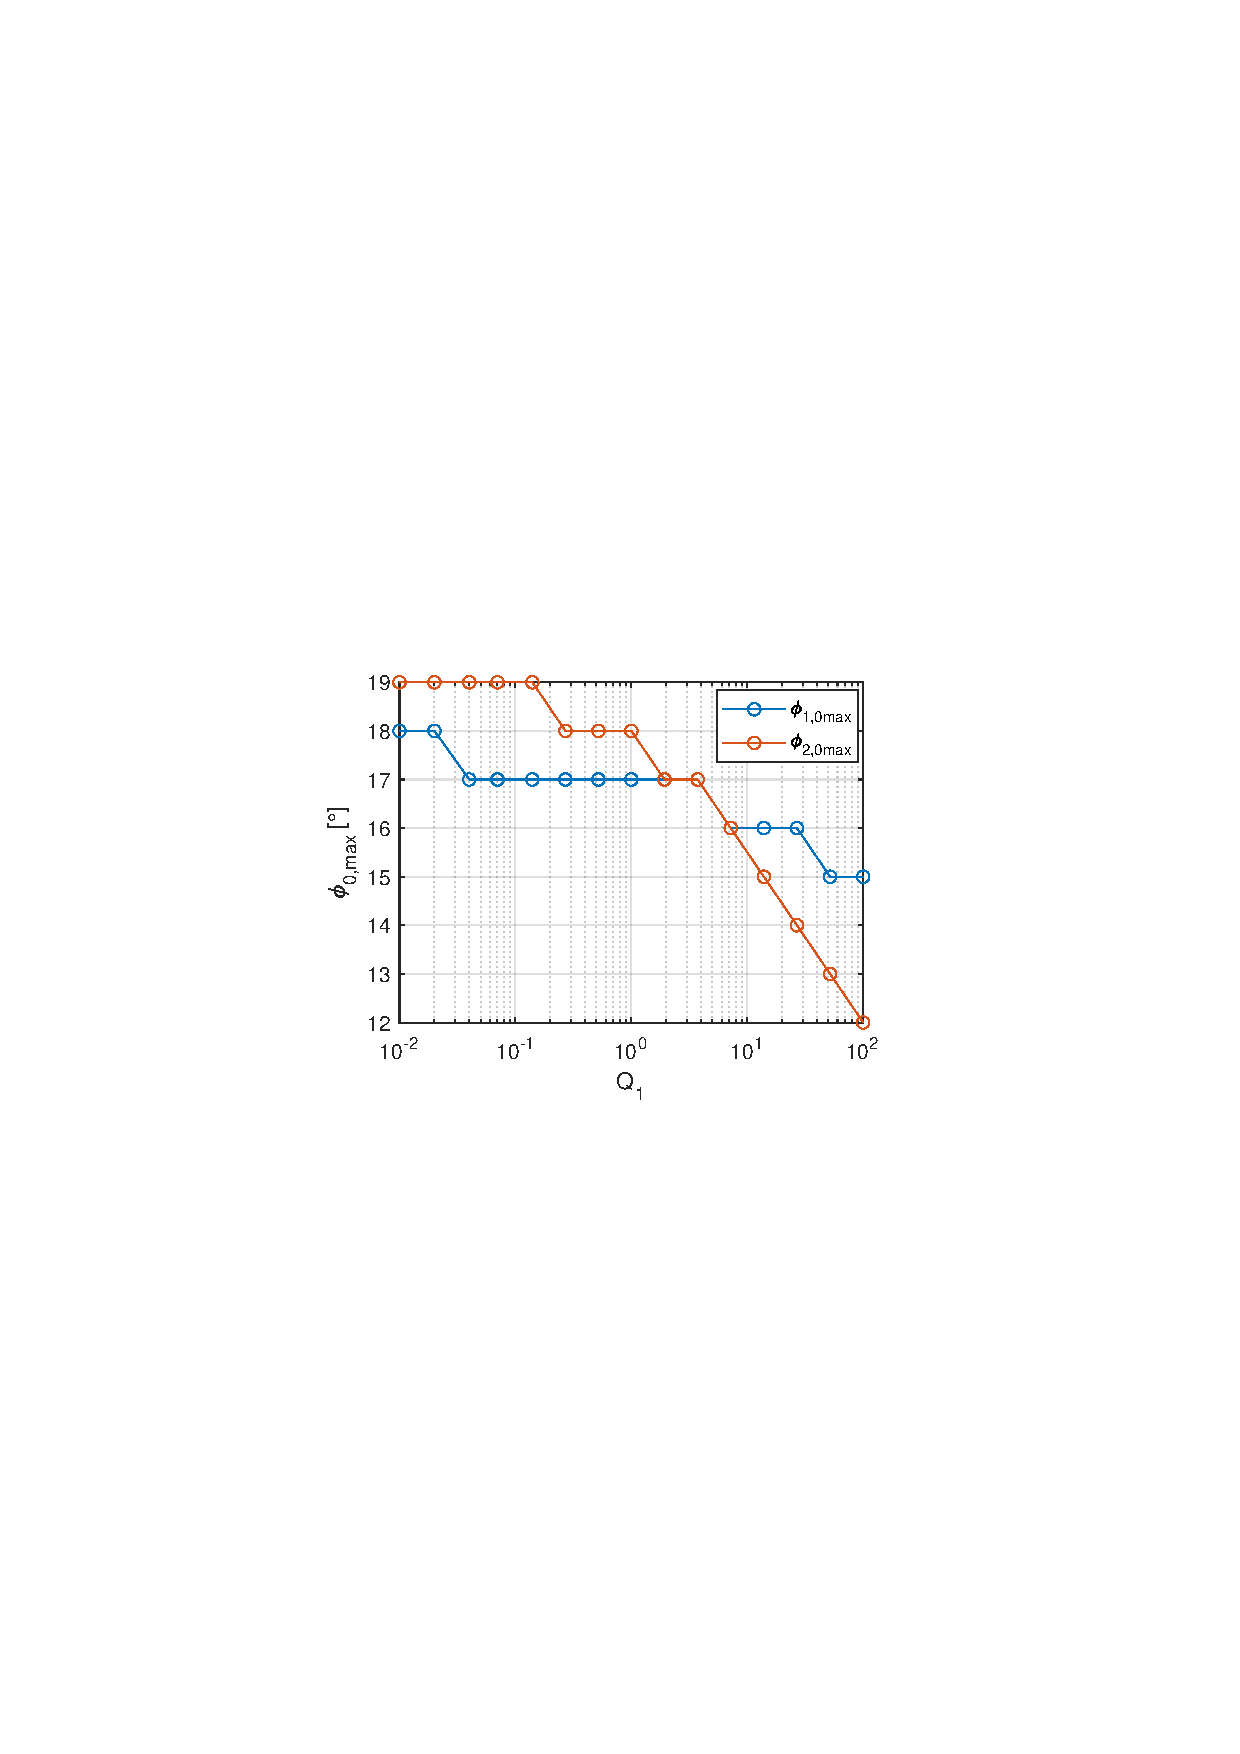
\includegraphics[width=0.55\textwidth]{Bilder/QRVariation/ap4/q1 phi12.pdf}
		\caption{Maximale Startwerte -- Variation von $Q_1$ bei \apv}
	\label{fig:qrap4q1}
\end{figure}

\begin{figure}[htbp]
	\centering
		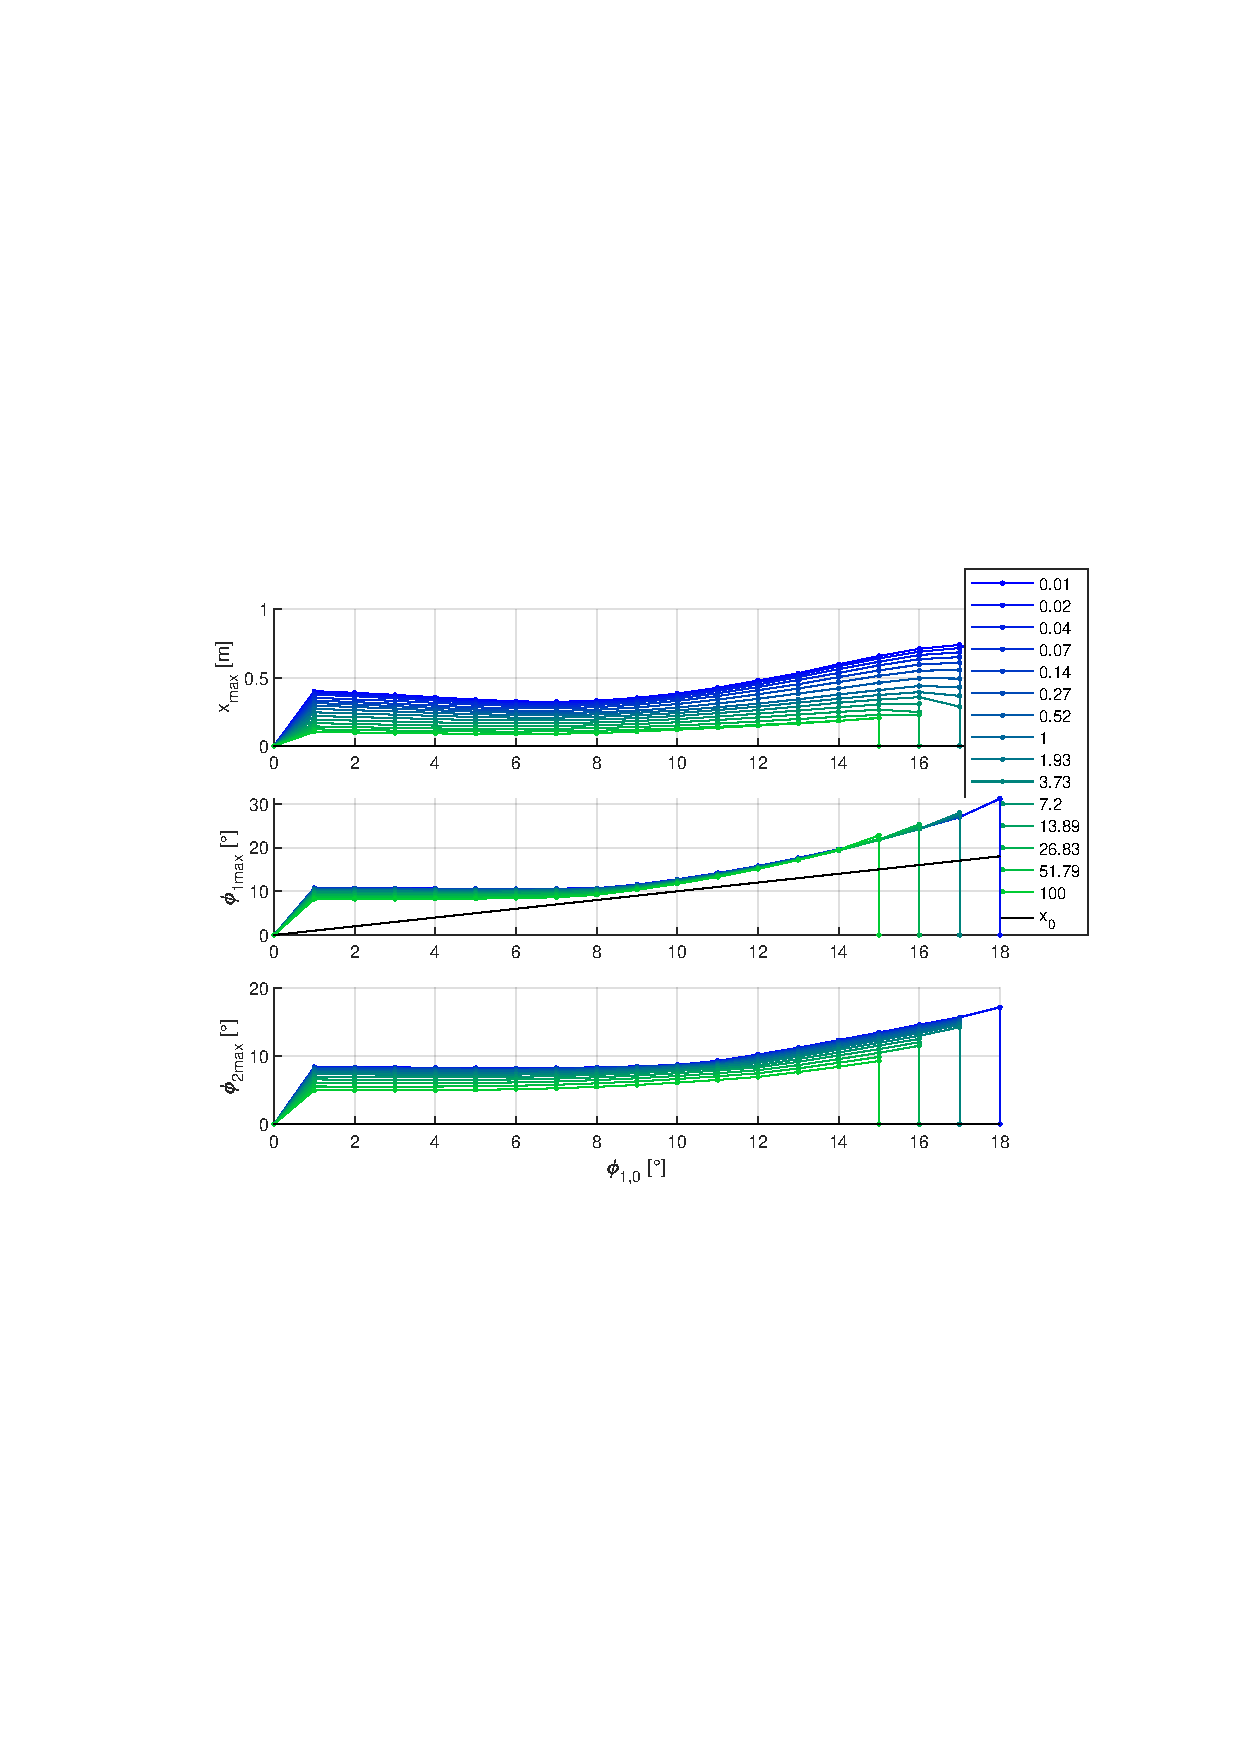
\includegraphics[width=0.85\textwidth]{Bilder/QRVariation/ap4/q1 phi1 m.pdf}
	\caption{Maximalabweichungen -- Variation von $Q_1$ bei \apv}
	\label{fig:qrap4q1m}
\end{figure}

Bei einer Variation von $Q_1$ an \apv\ ergibt sich für die maximalen Startwinkel der in \figref{fig:qrap4q1} dargestellte Verlauf.
Kleinere Werte von $Q_1$ führen tendenziell zu höheren möglichen Startwerten.
Allerdings sieht man an \figref{fig:qrap4q1m}, dass niedrigere Werte auch zu höheren Maximalabweichungen führen.
Daher wurde hier beispielsweise ein Kompromiss von $Q_1=1$ getroffen.


\subsection{Weitere Ergebnisse}

Insgesamt zeigte sich für R eine bessere Dynamik bei kleinen Werten, da dadurch die Stellgröße weniger stark gewichtet wird und somit höher sein darf.
Da geeignete Begrenzungs- und Anti-Windup-Maßnahmen vorhanden sind, stellt eine höhere Stellgröße grundsätzlich kein Problem dar.
R wurde für alle \ap e auf 0,01 gesetzt.

Die Werte $Q_1$ bis $Q_6$ wurden durch Auswerten aller Tests für alle \ap e in \texttt{AP\_QR\_20\_neu} angepasst und für das System \texttt{Ribeiro20} optimiert \siehe{\figref{fig:qrvglrib}}.
Die größten Auswirkungen zeigten sich bei $Q_1$. 
Meistens war der Einfluss der anderen Werte gering und brachte bei starker Erhöhung eine schlechtere Dynamik mit sich.
Bei \apv\ zeigte $Q_2$ und $Q_4$ einen deutlichen Einfluss.

Die Werte \texttt{AP\_QR\_20\_neu\_Beob} wurden für den Einsatz mit \beob\ optimiert.
Hierbei stellte sich heraus, dass für $Q_1$ generell größere Werte besser waren.
Besonders bei \apv\ mussten die Werte angepasst werden, damit das System einigermaßen stabilisiert werden kann.




\section{System Parameter Tests}\label{sec:x0sys}

Durch Verbesserung der Regelung und die systematische Optimierung der Reglerparameter konnte die Regelbarkeit des \dpd s deutlich verbessert werden und über einen größeren Bereich stabilisiert werden.
Trotzdem gibt es hierbei gewisse Grenzen, da die Eigenschaft der "`Regelbarkeit"' nicht nur vom Reglerentwurf, sondern auch vom System selbst abhängt.
Auch ist unklar, ob die durch die Simulation errungenen Ergebnisse direkt auf den realen Versuchsstand übertragbar sind.
Versuche mit dem \beob\ haben gezeigt, dass die \ze\ einen erheblichen Einfluss auf das Regelverhalten und die Stabilisierung hat.
Da am realen System weitere, nicht modellierte Effekte auftreten können, ist es von Vorteil, eine gewisse "`Reserve"' bezüglich der Regelbarkeit zu haben.


\subsection{Vorgehen}

Aus diesen Gründen wird in diesem Abschnitt die Regelbarkeit des Systems in Abhängigkeit der Systemparameter untersucht.
Somit wird die äußerste Schleife aus \figref{fig:regvorg} betrachtet.
Dabei ist zu beachten, dass jede Änderung am Streckenmodell \bzw deren Parametern Auswirkungen auf alle darunterliegenden Schleifen haben.
Der Regler muss am geänderten System erneut ausgelegt und berechnet werden.

Zudem muss theoretisch vor der Bewertung der Stabilisierbarkeit zunächst eine erneute Optimierung der Güteparameter stattfinden.
Da dieser Schritt jedoch schwer zu automatisieren ist und den Aufwand nochmals deutlich steigern würde, wird darauf verzichtet und es werden immer die im letzten Abschnitt optimierten QR-Parameter verwendet.
Somit muss im Hintergrund behalten werden, dass die Ergebnisse mit geänderten Systemparametern möglicherweise durch eine QR-Optimierung besser ausfallen können.

In diesem Abschnitt wird bei der Einflussanalyse der Systemparameter ausschließlich das neukonstruierte \dpd\ mit den Parametern \texttt{Ribeiro20} betrachtet \siehe{\tabref{tab:spdparams}}.
Erste Tests mit dem System am Versuchsstand haben eine deutlich schlechtere Regelbarkeit im Vergleich zum vorigen Aufbau gezeigt.
Wie bereits in \secref{subsec:spdparams} erwähnt, wird die erhöhte \crb\ dafür verantwortlich gemacht, weswegen diese besonders in den Fokus genommen wird.

Es werden die Parameter des \spds\ \siehe{\tabref{tab:abh}} variiert, um deren Einfluss auf die Stabilisierbarkeit zu analysieren und die Regelbarkeit zu erhöhen.
Dabei wird ein Parameter schrittweise geändert, alle anderen behalten ihren eigentlich Wert.
Demzufolge ist bei der Interpretation auch darauf zu achten, dass manche Parameter wie Masse, Trägheitsmoment und Schwerpunkt eigentlich voneinander abhängen.
Da außer den reinen Zahlenwerten der ermittelten Parameter keine weiteren Informationen über deren Zusammensetzung oder Modellierung vorliegen, werden die Parameter nur einzeln variiert.


\subsection{Anwendung in \ml}

Ähnlich wie bei der QR-Variation wird eine Funktion \texttt{SysParameter\_Variation} angelegt, die für einen gegeben Parametersatz den spezifizierten Parameter in dem angegebenen Bereich (hier meist linear) variiert.
Der Parameter wird so angegeben wie in \texttt{SchlittenPendelParams} definiert.
Für jeden Wert des Parameters wird das System und der Regler entsprechend initialisiert, anschließend werden die kritischen \xots s durchgeführt.
Ein Aufruf erfolgt beispielsweise mit:
	\[
	\texttt{SysParameter\_Variation(SchlittenPendelParams\_Ribeiro20(), 'm1', 0:0.2:2)}
\]
Weitere Information sind in der Funktion dokumentiert.
Zusätzlich befinden sich einige Aufrufbeispiele in \texttt{SysParameter\_Variation\_run.m}.



\subsection{Diagramme}

\subsubsection{Trägheits- und Geometrieparameter}


\figref{fig:sysvarm1} stellt die maximalen Startwerte der kritischen \xots s für die Variation der Pendelmasse $m_1$ im Bereich $0$ bis \valunit{2}{kg} dar.
Die gestrichelte Linie markiert den tatsächlichen Wert des Parameters (\texttt{Ribeiro20}).
Wie man sehen kann, hat der Parameter einen starken Einfluss auf das Stabilitätsgebiet, wobei die Tendenz \ap-abhängig ist.
Bei \apz\ führt eine \emph{geringere} Masse zu einem besseren Verhalten.
Vermutlich kann dadurch das erste Pendel schneller beschleunigt werden, wodurch auch größere Winkelabweichungen ausgeregelt werden können.
Im Gegensatz dazu führt bei \apd\ und \apv\ eine \emph{höhere} Masse zu einer besseren Regelbarkeit.
Bei diesen steht das erste Pendel, dessen Gelenk den nicht unerheblichen \crb skoeffizienten aufweist, oben.
Ein Erklärungsversuch besteht daher in der \crb: Durch die erhöhte Masse wird sie relativ gesehen kleiner und damit das System "`linearer"', was die bessere Regelbarkeit erklären könnte.

\newcommand{\scaleq}{0.62}
\begin{figure}[H]
	\centering
	\subfloat[\apaz]{ \includegraphics[scale=\scaleq]{Bilder/SysParam Variation/m1/AP2.pdf}	}
	\hfil
	\subfloat[\apad]{	\includegraphics[scale=\scaleq]{Bilder/SysParam Variation/m1/AP3.pdf}	}
	\\
	\subfloat[\apave]{ \includegraphics[scale=\scaleq]{Bilder/SysParam Variation/m1/AP41.pdf} }
	\hfil
	\subfloat[\apavz]{ \includegraphics[scale=\scaleq]{Bilder/SysParam Variation/m1/AP42.pdf}	}
	\caption{Maximale Startwerte -- Variation $m_1$}
	\label{fig:sysvarm1}
\end{figure}

\begin{figure}[H]
	\centering
	\subfloat[\apaz]{ \includegraphics[scale=\scaleq]{Bilder/SysParam Variation/m2/AP2.pdf}	}
	\hfil
	\subfloat[\apad]{	\includegraphics[scale=\scaleq]{Bilder/SysParam Variation/m2/AP3.pdf}	}
	\\
	\subfloat[\apave]{ \includegraphics[scale=\scaleq]{Bilder/SysParam Variation/m2/AP41.pdf} }
	\hfil
	\subfloat[\apavz]{ \includegraphics[scale=\scaleq]{Bilder/SysParam Variation/m2/AP42.pdf}	}
	\caption{Maximale Startwerte -- Variation $m_2$}
	\label{fig:sysvarm2}
\end{figure}

Die Variation von $m_2$ im Bereich $0$ bis \valunit{1}{kg} ist in \figref{fig:sysvarm2} dargestellt.
Hier zeigt sich für alle \ap e dieselbe eindeutige Tendenz: Je niedriger die Masse, desto besser ist die Stabilisierbarkeit.

Für die Schlittenmasse $m_0$ zeigt sich der erwartete Trend: Je größer die Masse, desto weniger lassen sich die \ap e stabilisieren \siehe{\figref{fig:sysvarm0}}.
Dies lässt sich hauptsächlich auf die \sgb\ zurückführen.

\renewcommand{\scaleq}{0.38}
\begin{figure}[p]
	\centering
	\subfloat[\apaz]{ \includegraphics[scale=\scaleq]{Bilder/SysParam Variation/J1/AP2.pdf}	}
	\hfil
	\subfloat[\apad]{	\includegraphics[scale=\scaleq]{Bilder/SysParam Variation/J1/AP3.pdf}	}
	\\
	\subfloat[\apave]{ \includegraphics[scale=\scaleq]{Bilder/SysParam Variation/J1/AP41.pdf} }
	\hfil
	\subfloat[\apavz]{ \includegraphics[scale=\scaleq]{Bilder/SysParam Variation/J1/AP42.pdf}	}
	\caption{Maximale Startwerte -- Variation $J_1$}
	\label{fig:sysvarJ1}
\end{figure}

\begin{figure}[p]
	\centering
	\subfloat[\apaz]{ \includegraphics[scale=\scaleq]{Bilder/SysParam Variation/J2/AP2.pdf}	}
	\hfil
	\subfloat[\apad]{	\includegraphics[scale=\scaleq]{Bilder/SysParam Variation/J2/AP3.pdf}	}
	\\
	\subfloat[\apave]{ \includegraphics[scale=\scaleq]{Bilder/SysParam Variation/J2/AP41.pdf} }
	\hfil
	\subfloat[\apavz]{ \includegraphics[scale=\scaleq]{Bilder/SysParam Variation/J2/AP42.pdf}	}
	\caption{Maximale Startwerte -- Variation $J_2$}
	\label{fig:sysvarJ2}
\end{figure}

Das Trägheitsmoment $J_1$ wird im Bereich von 0 bis zum doppelten Originalwert variiert \siehe{\figref{fig:sysvarJ1}}.
Es zeigt sich exakt der gegenteilige Trend im Vergleich zu $m_1$: Bei \apz\ verbessert ein \emph{höheres} Trägheitsmoment das Regelverhalten, bei den anderen ein \emph{niedrigeres}.
Die "`schnellere Drehbarkeit"' sorgt bei den \ap en mit dem ersten Pendel oben offenbar für bessere Stabilisierbarkeit.
Auch bei $J_2$ stellt sich der gegenteilige Trend zu $m_2$ ein: Ein höheres Trägheitsmoment \emph{erhöht} die maximale Startabweichung.

Bei $s_1$ zeigt sich eine ähnliche Tendenz wie bei $m_1$, wobei die Änderungen ab Werten größer des originalen gering sind \siehe{\figref{fig:sysvars1}}.

Der Einfluss von $s_2$ ist nur bei \apd\ deutlich und verbessert das Regelverhalten bei geringeren Werten.
Auch bei den anderen \ap en wird das Verhalten für geringere Werte etwas besser \siehe{\figref{fig:sysvars2}}.

Für $l_1$ zeigt sich bei \apz\ und \apd\ derselbe Trend: Je größer, desto schlechter die Stabilisierung \siehe{\figref{fig:sysvarl1}}.
Bei \apz\ kann die Stabilität mit geringeren Werten deutlich verbessert werden.
Bei \apv\ hingegen verschlechtern kleine Werte das Verhalten deutlich, während größer Werte als die originalen nicht zu einer Verbesserung führen.



\subsubsection{Reibungsparameter}

Die Parameter der viskosen Dämpfung zeigten im Bereich 0 bis doppelter Originalwert keinen oder nur einen geringen Einfluss.
Auch der \crb skoeffizient des Schlittens $\Fco$ zeigte keinen Einfluss, vermutlich weil die Schlittenreibung durch die Vorsteuerung sehr gut umgangen wird.

Anhand von \figref{fig:sysvarMc10} sieht man, dass \Mceo\ einen leicht negativen Einfluss hat, außer bei \apz, dort ist der Einfluss sogar positiv.
Wie schon in \figref{fig:vglpendelpar} festgestellt wurde, scheint es bei \apz\ weniger Probleme bezüglich der Gelenk-\crb\ zu geben und auch weniger Probleme mit \beob\ \siehe{\figref{fig:vglribze}}.
Da außerdem ein deutlicher Einfluss des \beob\ gerade am neuen System vorhanden ist \siehe{\figref{fig:vglribze}}, wird für \Mceo\ der Test ebenfalls mit \beob\ (und den dafür optimierten QR-Parametern) durchgeführt.
Bei \apv\ stellt sich heraus, dass schon geringfügig höherer Werte der Reibung das System überhaupt nicht mehr stabilisieren lassen.
Offensichtlich ist gerade die Kombination von erhöhter \crb, die das System auch in der Nähe des \ap es nichtlinear macht, und dem Einsatz des \beob s, welcher am linearen System ausgelegt ist und durch die \crb\ Schätzfehler entstehen, äußerst kritisch.

\figref{fig:sysvarMc10m} zeigt zudem die \ap abweichungen bei der Variation von \Mceo\ (\zm).
Hier lässt sich sehr gut der Einfluss auf den sich einstellenden Grenzzyklus insbesondere bei niedrigen Startwerten feststellen, wie er auch schon in \figref{fig:vglpendelpar} beobachtet wurde.
Bei $\Mceo=0$ beginnen die Kurven in 0 und verhalten sich anfangs linear.
Mit steigender Reibung wird jedoch die Dauerschwingung größer.
Besonders bei \apv\ sieht man, dass das System schon bei sehr kleinen Anfangswerten aus der Ruhe in den Grenzzyklus gebracht wird.
Bei \apz\ startet die Dauerschwingung zwar nicht bei 0, ist aber im Bereich von 2-3 bis etwa \valdeg{10} konstant.
Bei \apd\ ist der Einfluss geringer.

\renewcommand{\scaleq}{0.8}
\begin{figure}[htbp]
	\centering
	\subfloat[\apaz]{ \includegraphics[scale=\scaleq]{Bilder/SysParam Variation/Mc10/AP2.pdf}	}
	\hfil
	\subfloat[\apad]{	\includegraphics[scale=\scaleq]{Bilder/SysParam Variation/Mc10/AP3.pdf}	}
	\\
	\subfloat[\apave]{ \includegraphics[scale=\scaleq]{Bilder/SysParam Variation/Mc10/AP41.pdf} }
	\hfil
	\subfloat[\apavz]{ \includegraphics[scale=\scaleq]{Bilder/SysParam Variation/Mc10/AP42.pdf}	}
	\caption{Maximale Startwerte -- Variation \Mceo}
	\label{fig:sysvarMc10}
\end{figure}

\renewcommand{\scaleq}{0.6}
\begin{figure}[htbp]
	\centering
	\subfloat[\apaz]{ \includegraphics[scale=\scaleq]{Bilder/SysParam Variation/Mc10/m AP2.pdf}	}
%	\hfil
	\subfloat[\apad]{	\includegraphics[scale=\scaleq]{Bilder/SysParam Variation/Mc10/m AP3.pdf}	}
	\\
	\subfloat[\apave]{ \includegraphics[scale=\scaleq]{Bilder/SysParam Variation/Mc10/m AP41.pdf} }
%	\hfil
	\subfloat[\apavz]{ \includegraphics[scale=\scaleq]{Bilder/SysParam Variation/Mc10/m AP42.pdf}	}
	\caption{Maximalabweichungen -- Variation \Mceo\ in Abh. des Originalwerts ($0.0538$)}
	\label{fig:sysvarMc10m}
\end{figure}


Bei \Mczo\ zeigte sich bei einer Änderung bis zum 4-fachen Originalwert keinen Einfluss.


\subsection{Schlussfolgerungen zu Parameteränderungen}

Es stellt sich nun die Frage inwieweit die Pendelparameter verändert werden können, um das Regelverhalten zu verbessern.
Insbesondere sind die Parameter von Interesse, die ohne großen konstruktiven Aufwand angepasst werden können.

Aus den Verläufen der Trägheits- und Geometrieparameter kann noch keine direkte Schlussfolgerung zu Änderungen am System gezogen werden, da diese alle voneinander abhängen.
Wird beispielsweise eine zusätzliche Masse angebracht, ändert sich auch das Trägheitsmoment sowie der Schwerpunkt.
Daher müssen zuvor alle Parameter entsprechend angepasst und weitere Tests durchgeführt werden, bevor eine eindeutige Aussage getroffen werden kann.

Bei der Neukonstruktion \cite{chang} wurden an den Pendelstäben Gewindebohrungen realisiert, sodass zusätzliche Gewichte angebracht werden können, die für ein anderes Systemverhalten sorgen.
Erste Überlegungen sind daher, am ersten Pendel eine Masse anzubringen, dies laut Diagramm für \apd\ und \apv\ zunächst vorteilhaft ist.
Andererseits hat das dadurch höhere Trägheitsmoment einen negativen Einfluss, was für eine Anbringung nahe der Drehachse spricht.
Die Ergebnisse der Schwerpunktseinflusses sprechen bei \apd\ und \apv\ hingegen für eine Erhöhung des Schwerpunkts, also eine Anbringung näher am zweiten Gelenk. 
Aufgrund der gegensinnigen Tendenzen sind weitere Tests für bestimmte Ausführungen nötig.

Auch am zweiten Pendel könnten Massen angebracht werden.
Während das Diagramm der reinen Masse zunächst dagegen spricht, verbessert ein höheres Drehmoment die Stabilisierbarkeit.
Demzufolge könnte der Einfluss einer Masse an der Pendelspitze getestet werden.
Außerdem könnte die Masse durch Verkürzen des Pendels verringert werden.

Außerdem hat sich bei Variation der Fallbeschleunigung $g$ gezeigt, dass niedrigere Werte die Stabilisierbarkeit verbessern.
Daher könnte man überprüfen, ob sich der Versuchsstand zu einem Standort auf dem Mond verlegen lässt.